\chapter{Protein-protein Interaction Binding Site Prediction: DELPHI}
This chapter introduces our recent publication DELPHI \cite{li2020delphi} (\textcolor{red}{replace citation after paper accepted}), a deep learning based program for protein-protein interaction site prediction. We first describe the deep learning prerequisites used in DELPHI as well as the previous state-of-the-art methods. Then we describe both the algorithm and the implementation of DELPHI in details. Last, we compare DELPHI with nine state-of-the-art programs on five datasets showing that DELPHI outperforms other in all metrics. 
\section{Background}
\subsection{Deep Learning in Bioinformatics}
Deep Learning is a branch of machine learning \cite{goodfellow2016deep}. It is inspired by the structure and function of the brain called artificial neural networks. From a high level, any computational programs can be considered mathematical transformation on given inputs. Traditional programs handcraft these mathematical computations while machine learning algorithms learn them. The mathematical transformation is learned from known examples, generally without being programmed with specific rules.

For example, in the Handwritten Digit Recognition problem, researchers used to design specific rules to to capture the characteristics of each number. While in deep learning, only the structure of a network is built. The network "learns" the ability of telling a handwritten number by seeing a large amount of labeled data as shown in Fig. \ref{fig_dig_rec}.
\begin{figure}[!h]
\begin{center}
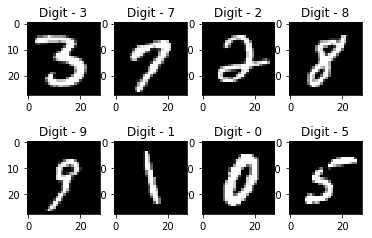
\includegraphics[width = 9cm]{img/digit_recog.png}
\caption{The labeled data in the Handwritten Digit Recognition problem. Each handwritten number (inside the black boxes) is labeled with its true value (above each handwritte number). From medium.com \label{fig_dig_rec}}
\end{center}
\end{figure}
%We illustrate this using a simple house price predictor as an example shown in Fig. \ref{fig_house_price}. Assume size, number of bedrooms, zip code, and wealth are the four factors to determine the house price. Traditional method need to hard code the mathematical relationship between the four inputs and the final predicting price y. For example, a linear function with a weight $\theta$ to each factor $x_i$. Written in vector notation is $y=\theta^Tx$. $\theta$ in this case is handcrafted. In contrast, deep learning methods define the computation flow (edges) between each value (nodes). The actual computation is learned by seeing sample data, for example 100 known house price and their four attributes. 
% \begin{figure}[!h]
% \begin{center}
% 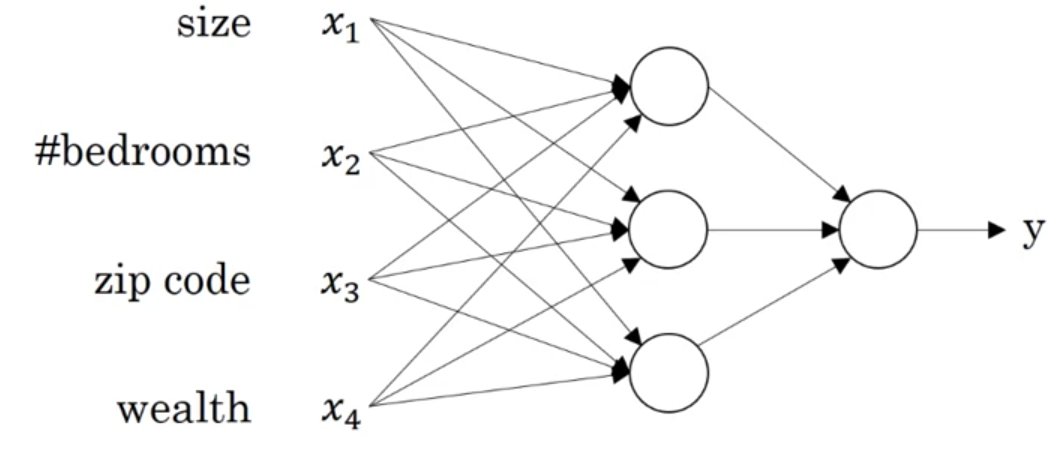
\includegraphics[width = 9cm]{img/house_price.png}
% \caption{Example of predicting house price using computational methods. The x1 - x4 indicate the four factors in determine the house price. Circles indicate computations and edges indicate data flows in the computations. \label{fig_house_price}}
% \end{center}
% \end{figure}

Many bioinformatics problems have been transformed into well defined mathematical problems. For example, sequence alignment, tree comparison, similarity search etc.These problems often have good algorithmic solutions. However, there are also large amount of bioinformatics problems are far from understanding, and many of them are fundamental problems such as coding region identification, structure prediction, interaction identification, biomedical image classification \cite{larranaga2006machine}. The biggest obstacle of solving these problems are the underlying mechanism is biologically complicated so that even biologists can not give definitive explanation of the factors and how they are related. 

With the increasing amount of biological data, more and more hard biological problems have been attempted to solve using deep learning methods. As shown in Fig. \ref{fig_deelLearning_papers}, since early 2010s, the number of deep learning bioinformatics methods has increased drastically. This is due to several reasons. First, significant amounts of biomedical data have been accumulated which enables significant performance improvement deep learning methods. For example, as shown in Fig. \ref{fig_pdb_stats}, from year 2000 to 2020 April, The total number of PDB \cite{berman2002protein} released structures increased from 13,589 to 162,529, which is almost 12 times bigger as two decades ago. As shown in Fig. \ref{fig_data_performance}, the performance of deep learning methods generally increases with more data while traditional methods reach its maximum performance after being fed with certain amount of data. Second, great amount of efforts have been made in deep learning software hardware co-design to accelerate the deep learning process especially for accelerating training. On the software side, numerous deep learning frameworks and compilers have been released and well maintained. Many of them of opensource programs with tight community integration. Popular frameworks include Google's Tensorflow \cite{tensorflow2015-whitepaper}, PyTorch \cite{NEURIPS2019_9015}, Caffe \cite{jia2014caffe}, high level API libraries like Keras \cite{chollet2015keras}, and recently opensourced MindSpore \cite{liao2019davinci} from Huawei. Compiler optimizations have also been explored greatly. For instance, Google's MLIR \cite{lattner2020mlir} project aims to unify the deep learning intermediate representation so that frontend APIs and the hardware can integrate more smoothly. The TVM \cite{chen2018tvm} project aims to automate the kernel implementation on various hardware.  These software makes deep learning easy to use and efficient during runtime. On the hardware side, general purpose CPU was initially used for deep learning computation. Soon GPU became very popular because of its vector computation unit that greatly accelerates the vector computations in deep learning. Recent years, specialized hardware focusing on the cube unit have also been developed by major companies. Cube unit performs matrix multiply in a single cycle which further accelerates deep learning computations. Well known examples include Google's Tensor Processing Unit (TPU), chips produced by Habana Lab (acuired by Intel), and Huawei's Ascend chips etc. As shown in Fig. \ref{fig_hardware_speedup}, the full setup of TPU could potentially speedup 200 times of the training on Resnet50. Third, biological problems are often too complicated for hand-crafted algorithms. Deep learning on the other hand can takes advantage of the growing number of data and captures the underlying patterns buried in high dimentionla data that human cannot.  Fourth, the influence of events and completions has attracted many researchers into the field of AI. To name a few, in ImageNet Large Scale Visual Recognition Challenge in 2012, AlexNet \cite{krizhevsky2012imagenet} ranked the first place and surpassed the second place by a huge 10.8\% margin. In October 2015, AlphaGo \cite{silver2017mastering} beat the professional Go player Lee Sedol on a full-sized board. Deepmind’s AlphaFold \cite{senior2020improved} won CASP13 protein-folding competition in 2018. 
\begin{figure}[h!]
\begin{center}
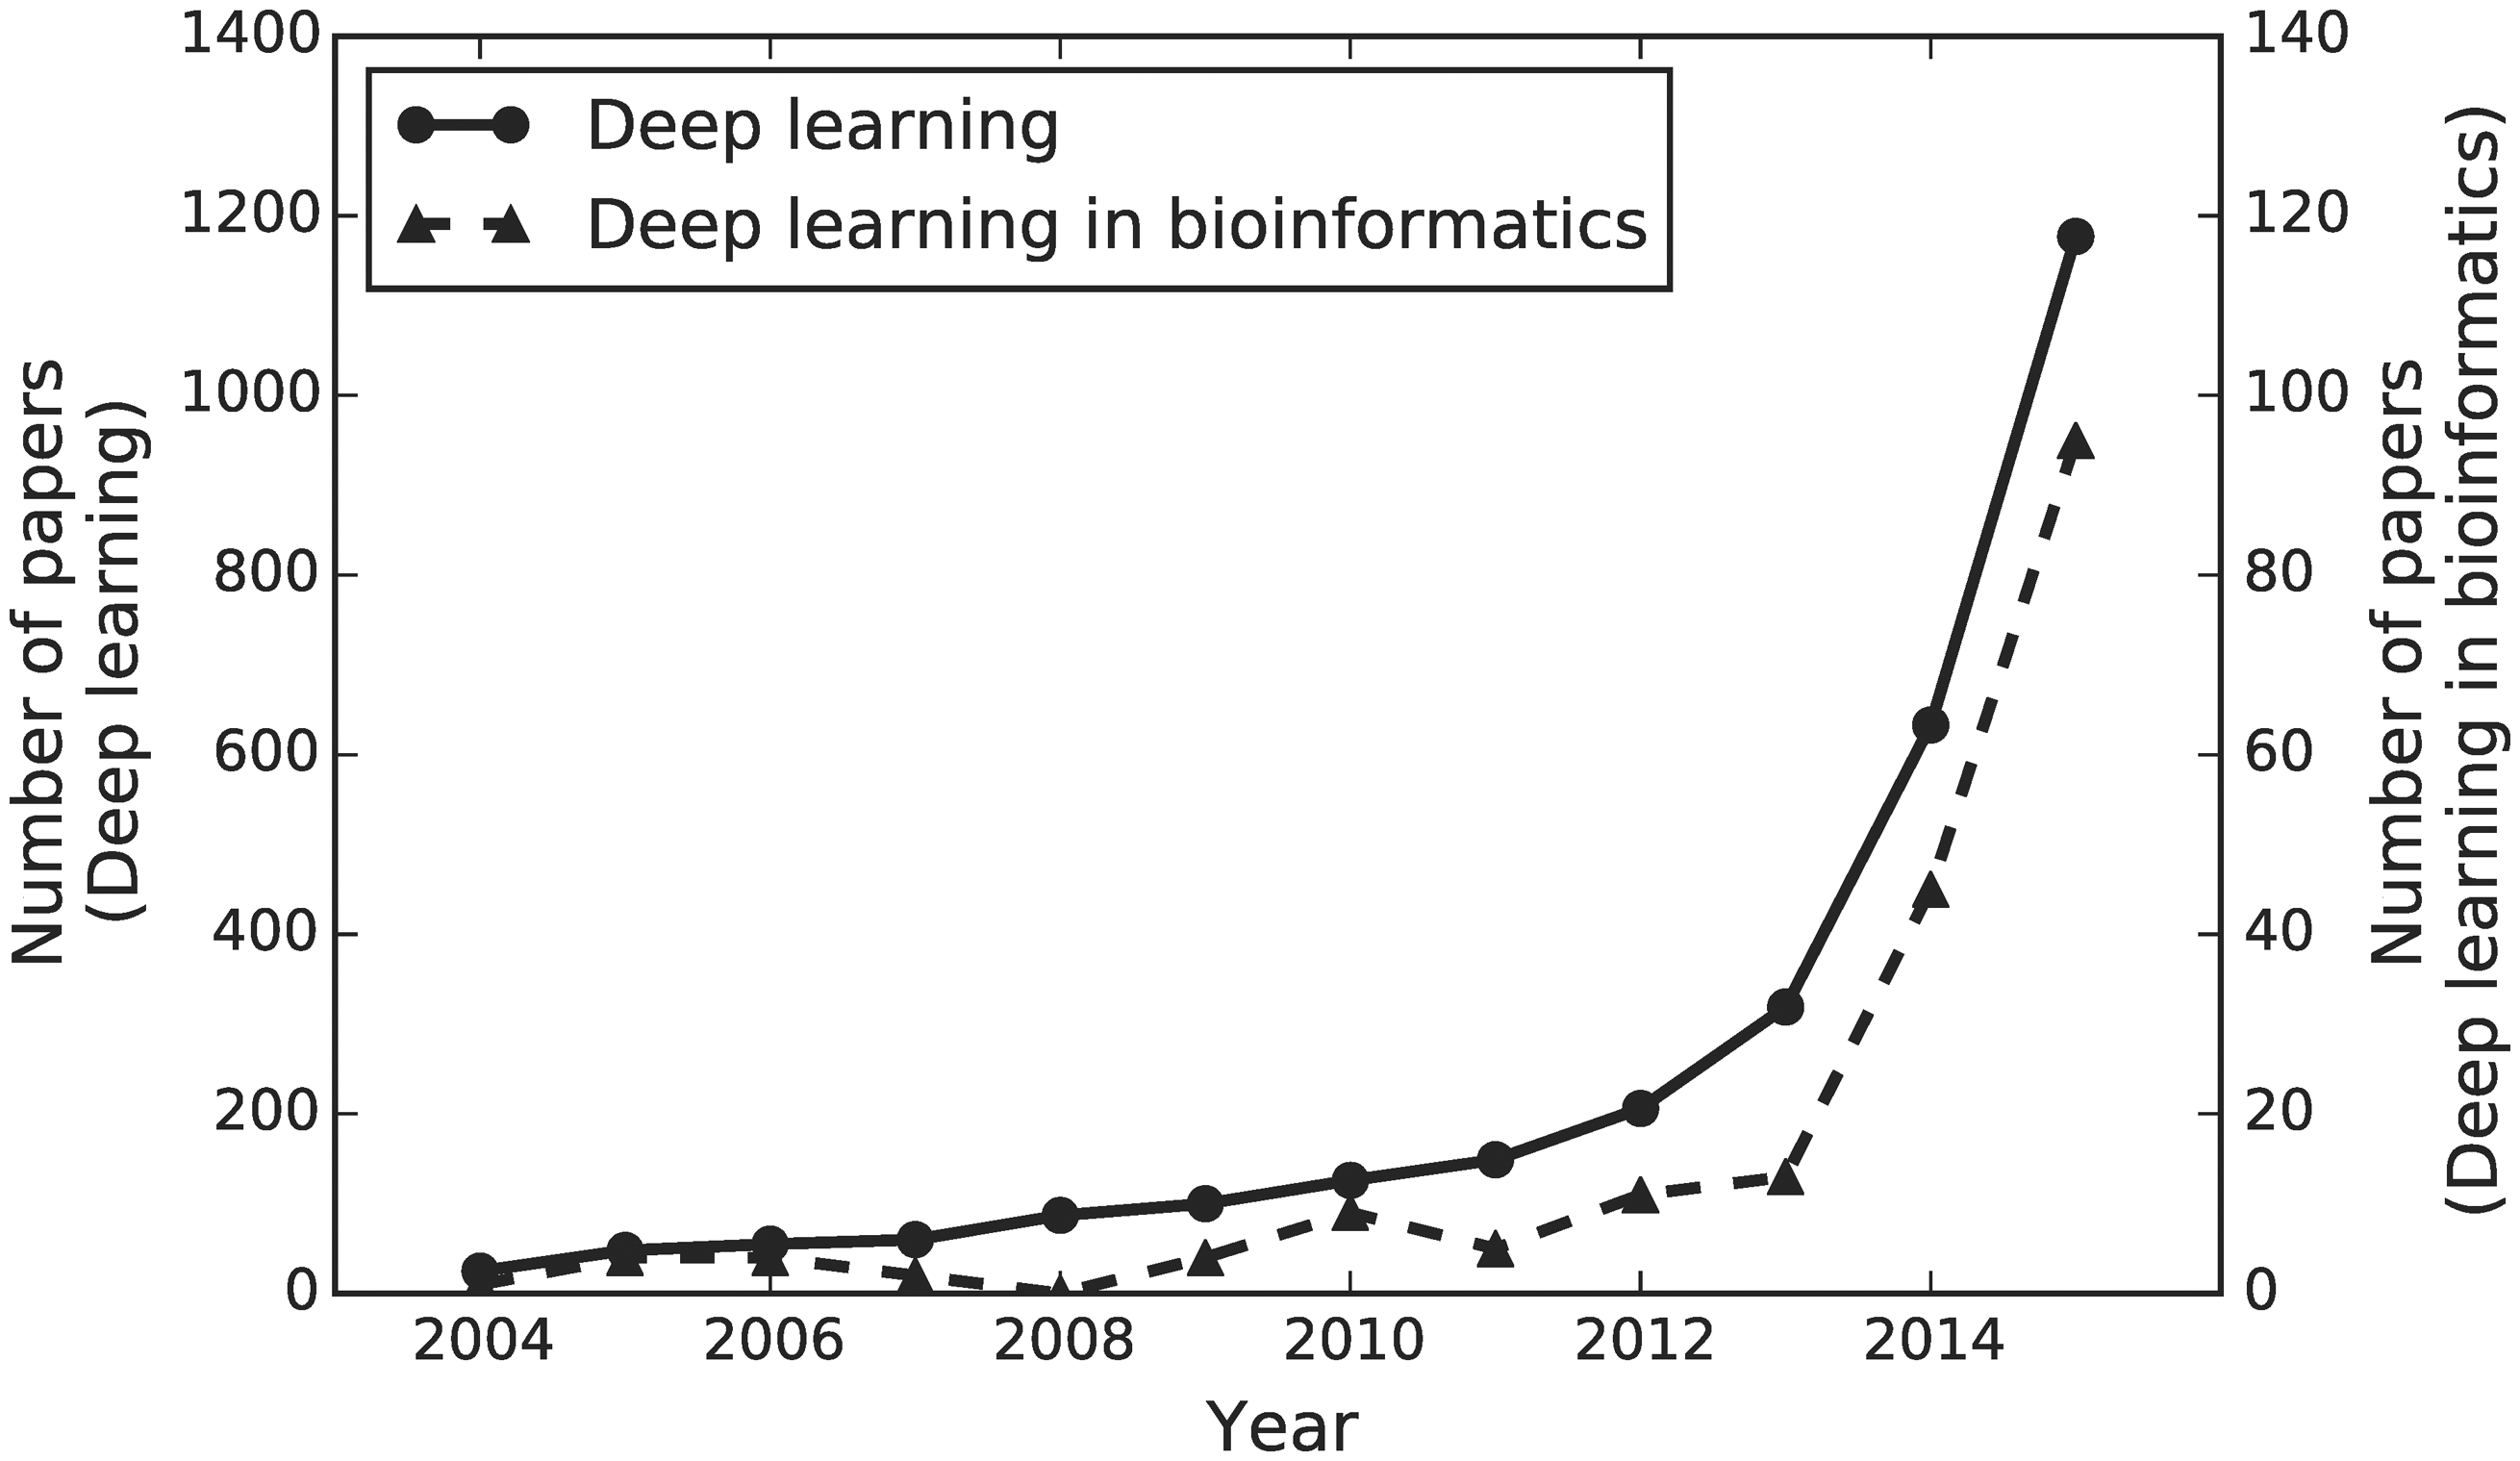
\includegraphics[width = 9cm]{img/deepLearning_in_bioinfo.png}
\caption{Approximate number of published deep learning and deep learning bioinformatics papers by year. From \cite{min2017deep}.  \label{fig_deelLearning_papers}}
\end{center}
\end{figure}

\begin{figure}[!h]
\begin{center}
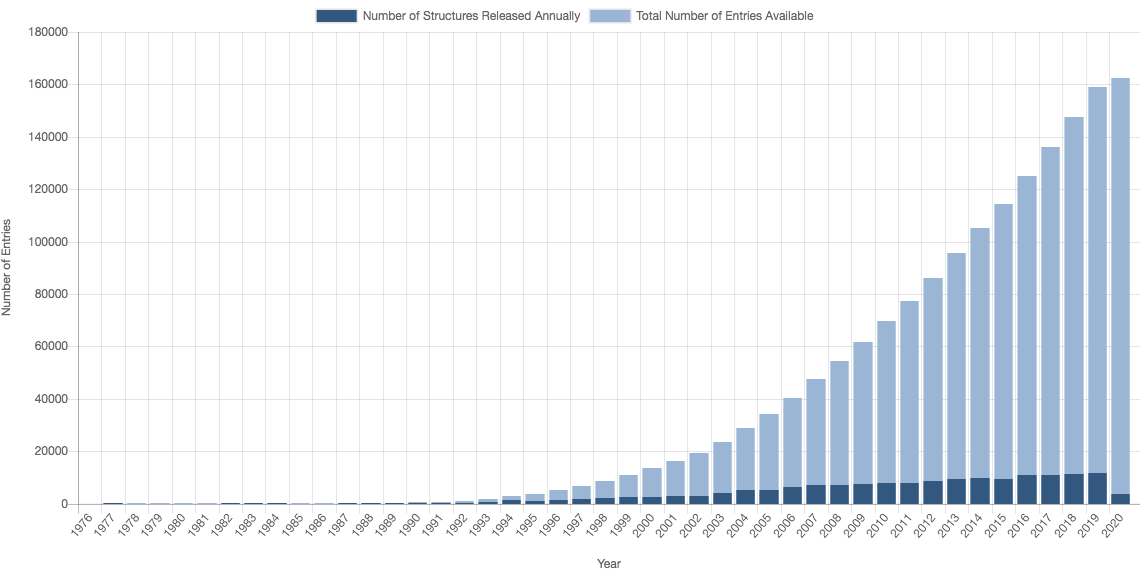
\includegraphics[height = 6cm, width = 9cm]{img/pdb_stats.png}
\caption{PDB Statistics: Overall Growth of Released Structures Per Year. From rcsb.org \cite{berman2002protein} \label{fig_pdb_stats}}
\end{center}
\end{figure}

\begin{figure}[!h]
\begin{center}
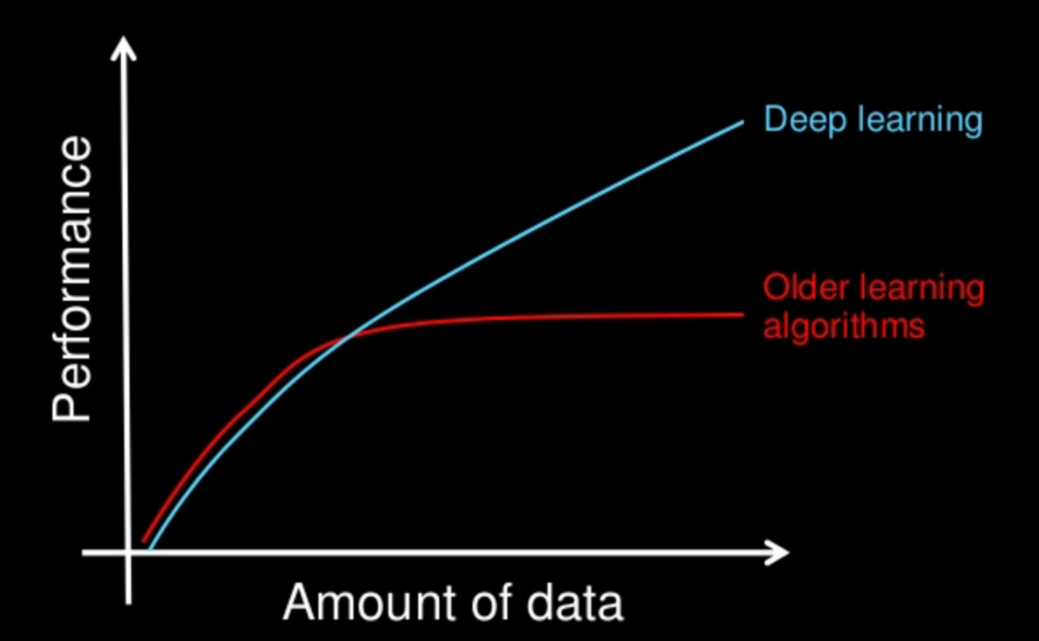
\includegraphics[height = 7cm, width = 9cm]{img/data_deeplearning.png}
\caption{Learning performance with the increament of data . From deepai.org/  \label{fig_data_performance}}
\end{center}
\end{figure}

\begin{figure}[h!]
\begin{center}
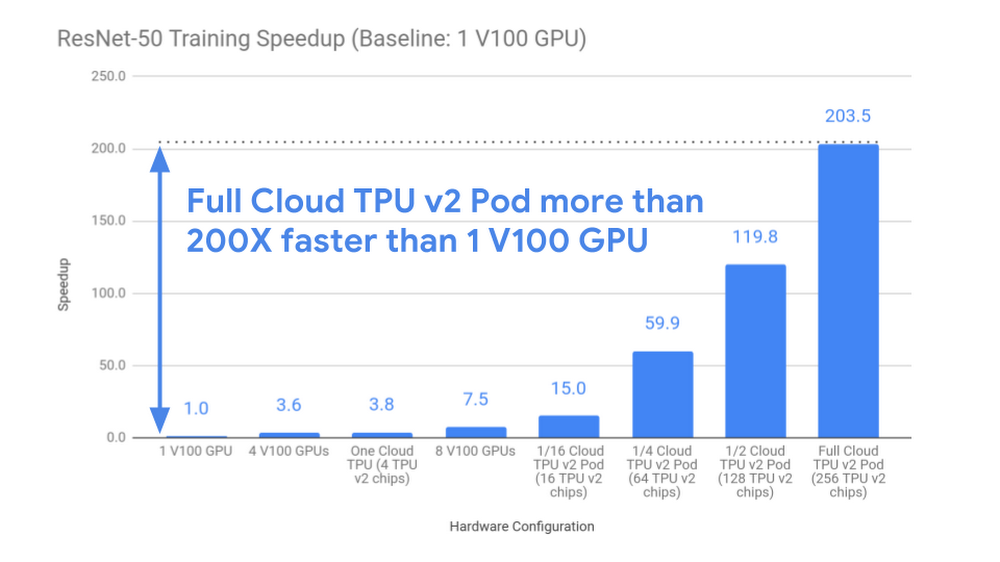
\includegraphics[height = 6cm, width = 13cm]{img/hardware_speedup.png}
\caption{Google's TPU speedup on Resnet50 training. From cloud.google.com/tpu \label{fig_hardware_speedup}}
\end{center}
\end{figure}

In the area of PPI prediction and PPI binding site prediction, most of methods published within a past decade are machine learning based. Seeing the trend, we designed and implemented our program DELPHI using deep learning techniques as well.

\subsection{Basic Notions and Definitions}
\subsubsection{Deep neural networks}
Neural networks learn complex mathematical transformations using layers of neurons. Fig. \ref{fig_mlp} shows the classic structure of a multilayer perceptron (MLP). It consists of at least three layers. The input layer, the output layer, and the hidden layers. The input layer is the initial state of the data. In bioinformatics, often raw data such as DNA or protein sequences is converted to features representations like embedding or position-specific scoring matrix (PSSM). Sequence itself contains useful but often limited information and needs to be represented further using features. The input layer is then passed to hidden layers for further computation. The term “deep learning” comes from the fact that the number of the hidden layers is big.
\begin{figure}[h!]
\begin{center}
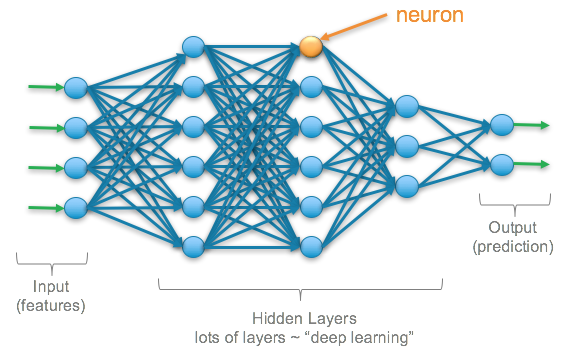
\includegraphics[width = 13cm]{img/multiplayer_perceptron.png}
\caption{Multilayer perceptron (MLP). An MLP must have at least three layers: the input layer, a hidden layer and the output layer. From medium.com \label{fig_mlp}}
\end{center}
\end{figure}

The term neuron, or often referred to as perceptron, means a mathematical function. As shown in Fig. \ref{fig_neuron}, a neuron takes in one or more inputs and apply mathematical functions on them and obtain an output called hypothesis. Each input is multiplied by a weight with the intuition of weighing the importance of each input.
% one or more inputs are multiplied by values called weights and then combined together with a bias value to better fit the model. Simple models often Linear Regression and Logistic Regression. Linear regression is a linear function while logistic regression is non linear.
\begin{figure}[h!]
\begin{center}
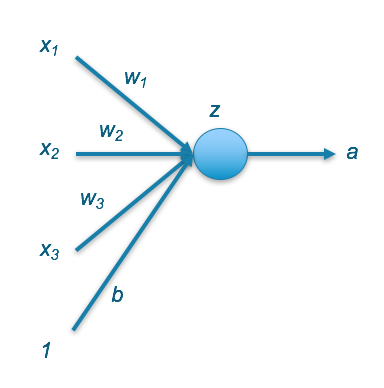
\includegraphics[height = 6cm, width = 7cm]{img/neuron.png}
\caption{A neuron in deep learning networks. $x_1$ - $x_3$ are inputs. $b$ is the bias value. $w_1$ - $w_3$ are the weights. $Z$ is the value before applying activation functions. $a$ is the final output value.\label{fig_neuron}}
\end{center}
\end{figure}
% For inputs $x1, x2 ... xi$, the vector notation for Linear Regression and Logistic Regression are \ref{equ_linear_regression} and \ref{equ_logistic_regression} respectively where $h_\theta(x)$ are the output, also known as hypothesis, $\theta^T$ is the weights and b is the bias. 
% \begin{equation}
% h_\theta(x)=\theta^Tx + b \label{equ_linear_regression}
% \end{equation}

% \begin{equation}
% h_\theta(x)=\frac{1}{1+e^{-\theta^Tx}} \label{equ_logistic_regression}
% \end{equation}
After calculating the hypothesis, an non-linear function is often applied to it, and this is called an activation function. The intuition of the the term "activation" is that each neuron calculates the hypothesis of inputs and if the result is greater than a threshold, then the neuron activates and send a signal to the next neuron. Popular activation function include Sigmoid, tanh, ReLU, LeakyReLU, Maxout, ELU \cite{goodfellow2016deep}. Their function and plots are shown in Fig. \ref{fig_activation_func}.
\begin{figure}[h!]
\begin{center}
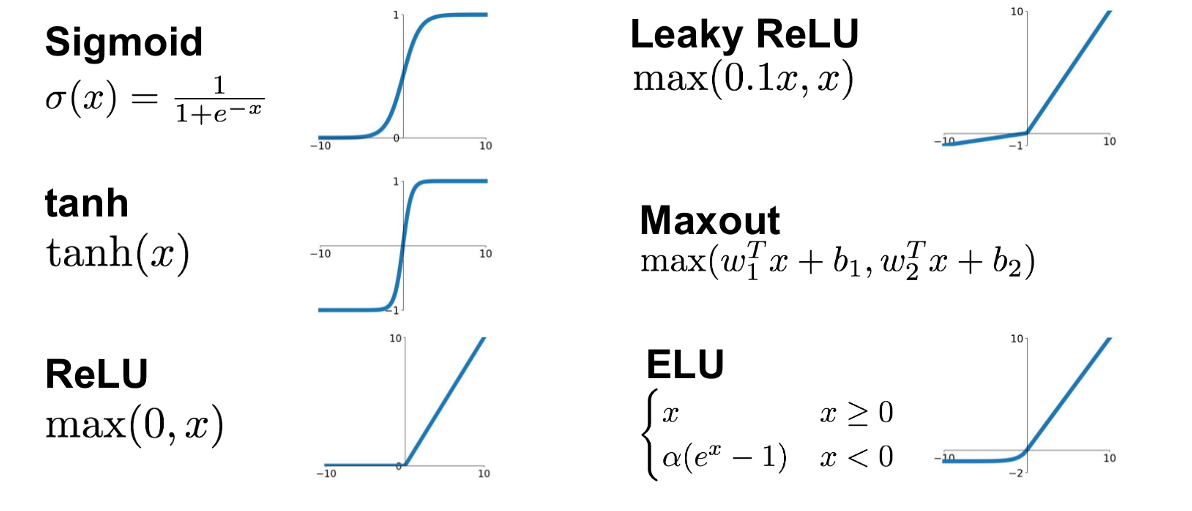
\includegraphics[width = 13cm]{img/activation_function.png}
\caption{Popular activation functions and their plots.\label{fig_activation_func}}
\end{center}
\end{figure}

\subsubsection{Training}
The output of a network may not be able to predict the true vale of a sample. The weights in network need to be tuned to achieve better prediction. This process is called training a neuron network.

First, we need to measure how well the current network is doing by having calculating the the difference, or cost, between the current predicted value and the true value of the output. This is done by having a loss function. A commonly used loss function for is least square which is shown in Equation \ref{equ_least_square} in vector notation, where $J(\theta)$ is the cost, $h_\theta(x^{(j)})$ is the predicted value or the hypothesis, $y^{(j)}$ is the ground truth, and $m$ is the number of samples. Other popular loss functions include mean squared error, cross-entropy, hellinger distance, logcosh etc \cite{goodfellow2016deep}.
\begin{equation}
J(\theta)=\frac{1}{2}\sum^m_{j=1}(h_\theta(x^{(j)}) - y^{(j)})^2
 \label{equ_least_square}
\end{equation}

The training process aims to minimize the loss function. The weights will be adjusted gradually. The most popular algorithm for this is gradient descent. As shown in Fig. \ref{fig_gradient_descent}, the initial value of the weight $w$ is the left-most blue circle. The yellow point on the plot is the best choice of the weight because it renders the minimal loss. Denoting in vector representation, given an initial guess for the weights $\theta$, the weights are updated such that the cost moves in the direction of steepest descent \cite{robbins1951stochastic}. The updated weights $\theta_j$ are computed as in Equation \ref{equ_gradient_descent}.
\begin{equation}
\theta_j=\theta_j - \alpha\frac{\partial}{\partial\theta_j}J(\theta)
 \label{equ_gradient_descent}
\end{equation}

\begin{figure}[h!]
\begin{center}
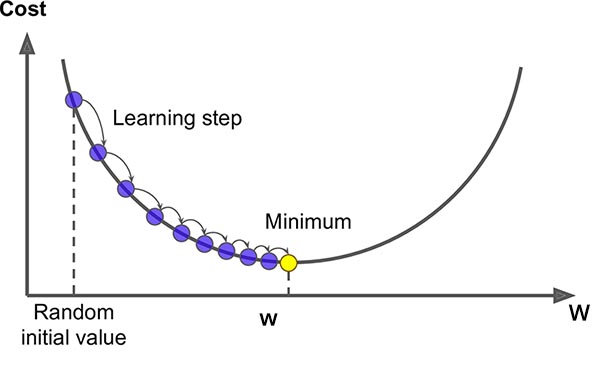
\includegraphics[width = 11cm]{img/gradient_descent.jpg}
\caption{The illustration of gradient descent. The x-axis is the value of the weight, and the y-axis is the corresponding cost. The aim is to choose a $w$ that minimizes the cost. \label{fig_gradient_descent}}
\end{center}
\end{figure}

In Keras, training can be done using the Model Class API as follows.
\begin{lstlisting}[language=python,frame=single]
model.fit(x = input_data, y = labels, epochs=10, ...)
\end{lstlisting}

\subsubsection{Inference}
After training the network, all the weights are fixed and the network is ready to predict on new data. This predicting process is called inference. Fig. \ref{fig_train_vs_infer} illustrates the process of the training and inference process of a neuron network. Performing inference on a network is significantly faster than training that network.
\begin{figure}[h!]
\begin{center}
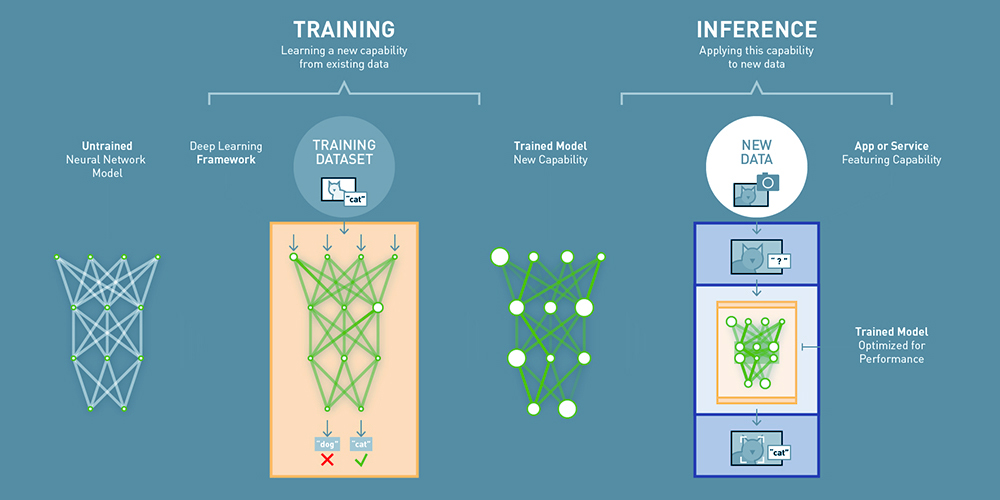
\includegraphics[width = 13cm]{img/train_inference.jpg}
\caption{The illustration of training and inference processes. \label{fig_train_vs_infer}}
\end{center}
\end{figure}

In Keras, inference can be done using the Model Class API as follows.
\begin{lstlisting}[language=python,frame=single]
model.predict(x = input_data, ...)
\end{lstlisting}

\subsubsection{Convolutional Neural Networks}
One of the shiniest algorithms in deep learning is Convolutional Neural Network (CNN). In recent decades, it has led the major advancements in the field of computer vision, image and video classification, media recreation, and recommendation systems. CNN is the core layer of many state-of-the-art deep learning networks such as AlexNet (2012) \cite{krizhevsky2012imagenet}, ZFNet (2013) \cite{zeiler2014visualizing}, GoogLeNet/InceptionV1 (2014) \cite{szegedy2015going}, VGGNet (2014) \cite{simonyan2014very}, ResNet50 (2015) \cite{he2016deep}, Xception (2016) \cite{chollet2017xception}, ResNeXt-50 (2017) \cite{xie2017aggregated} and many of their variants. The basic building blocks of a CNN are convolutional layers, pooling layers, and fully connected layers, as shown in Fig. \ref{fig_CNN}. 

\begin{figure}[h!]
\begin{center}
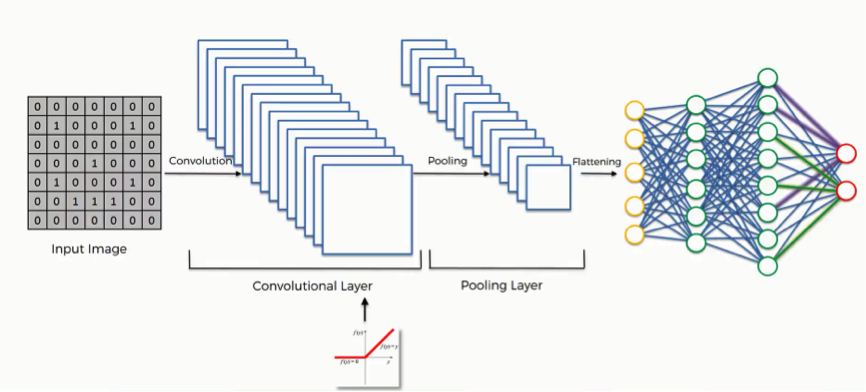
\includegraphics[width = 13cm]{img/convlution.png}
\caption{The basic building blocks of a Convolutional Neural Network: convolutional layers, pooling layers, and fully connected layers. From superdatascience.com \label{fig_CNN}}
\end{center}
\end{figure}

The computation of a convolution applied on a 2D image is as follows. As shown in Fig. \ref{fig_Conv2d}, the input is an image, often called a feature map, which is represented as a 2D matrix $I$. A sliding window, in this example of size 3x3 is placed on top and shifted through the entire image. Elementwise multiplication is conducted on each sub-matrix and another matrix called filter or kernel, denoted as $K$. The summation of the elementwise multiplication is placed as one value in the output matrix $I*K$. The values in the kernel matrix is learned during training. The intuition of the convolution operation is to extract the higher level features such as edges, from the input image. A CNN is not limited to one layer of convolution operation. Each convolution layer is meant to extract more abstract information from its previous input.
\begin{figure}[h!]
\begin{center}
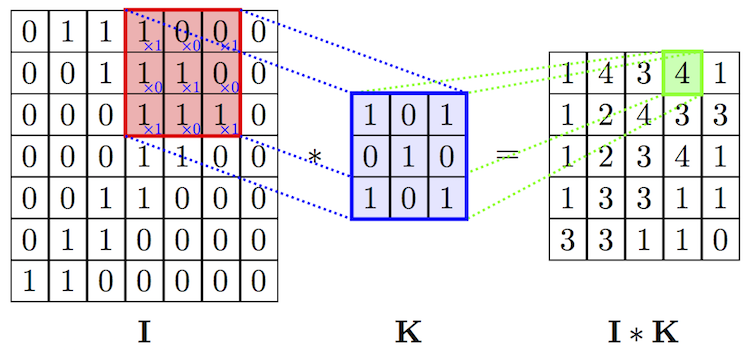
\includegraphics[width = 13cm]{img/convolution_computation.png}
\caption{The computation inside a convolution operation. A sliding window is applied on the input image $i$. Each window multiplies the kernel matrix $K$ elementwise. The summation of the product is placed as one value in the output matrix. For example, the summation of the elementwise multiplication between a sub-matrix (red) and the kernel matrix (blue) is 4 (green). This computation is $1*1+0*0+0*1+1*0+1*1+0*0+1*1+1*0+1*1 = 4$.   \label{fig_Conv2d}}
\end{center}
\end{figure}

The convolution layer can be implemented in Keras in either 1D or 2D depending on the shape of the input tensor.
\begin{lstlisting}[language=python,frame=single]
keras.layers.Conv2D(filters, kernel_size, ...)
\end{lstlisting}

The convolution layer is often followed by a pooling layer. The Pooling layer is responsible for reducing the size of the extracted features from the previous convolution operation. As shown in Fig. \ref{fig_pooling}, there are two popular types of pooling operations: max pooling and average pooling. Max Pooling returns the maximum value from the portion of the input, and average pooling returns the average value. In most applications, max pooling has a better performance than average pooling. One interpretation is that the max pooling operation performs noise suppressant by discarding all noisy values while average pooling retaining them.
\begin{figure}[h!]
\begin{center}
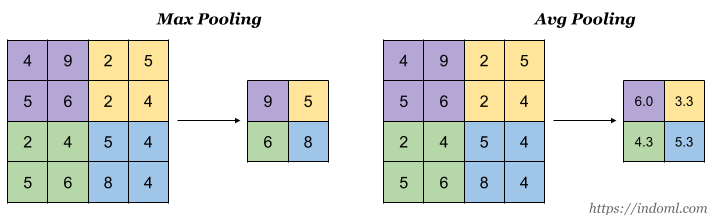
\includegraphics[width = 13cm]{img/pooling.png}
\caption{Examples of the pooling operation. The input matrix is divided into four sub-matrces, and each of them is performed a pooling operation. For example, the purple sub-matrix has four values 4, 9, 5, 6. Max pooling computes their max value, which is 9, and the average pooling computes the average, whcih is 6. From towardsdatascience.com \label{fig_pooling}}
\end{center}
\end{figure}

The intuition behind pooling layers is that the reduced image still contains the dominant features that are adequate to represent the original image. As shown in Fig. \ref{fig_pooling_blurry}, the image after the maxpooling operation (right) is reduced in size comparing to its input image (left), but it is still clear that the image content is a car. 
\begin{figure}[h!]
\begin{center}
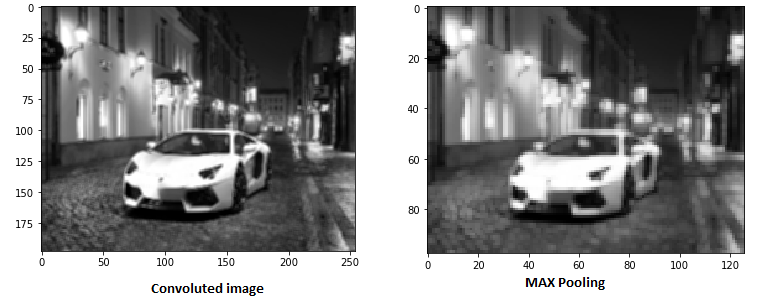
\includegraphics[width = 13cm]{img/pooling_blurry.png}
\caption{The intuition of the pooling operation. The original image after a convolution operation is on the left, and the image after the max pooling operation is on the right. From analyticsvidhya.com \label{fig_pooling_blurry}}
\end{center}
\end{figure}

In Keras, pooling layers can be implemented using the layers API.
\begin{lstlisting}[language=python,frame=single]
# Max Pooling
keras.layers.MaxPooling2D(pool_size=(2, 2), ...)
# Average Pooling
keras.layers.AveragePooling2D(pool_size=(2, 2), ...)
\end{lstlisting}

The last layer(s) of a CNN is usually fully connected layers. The role of a fully connected layer is to transform the results of the convolution or pooling operations to one or few values. It is called fully connected layers because every neuron is connected to all the neurons in the next layer. As shown in Fig. \ref{fig_fc}, each node in a fully connected layers is the weighted summation of all its input. The weighs are trained during training. The computation denoted in vector notation is shown in Equation \ref{equ_linear_regression} where $h_\theta(x)$ are is the outputs, $x$ is the inputs, $\theta^T$ is the weights and b is the bias. 
\begin{equation}
h_\theta(x)=\theta^Tx + b \label{equ_linear_regression}
\end{equation}
\begin{figure}[h!]
\begin{center}
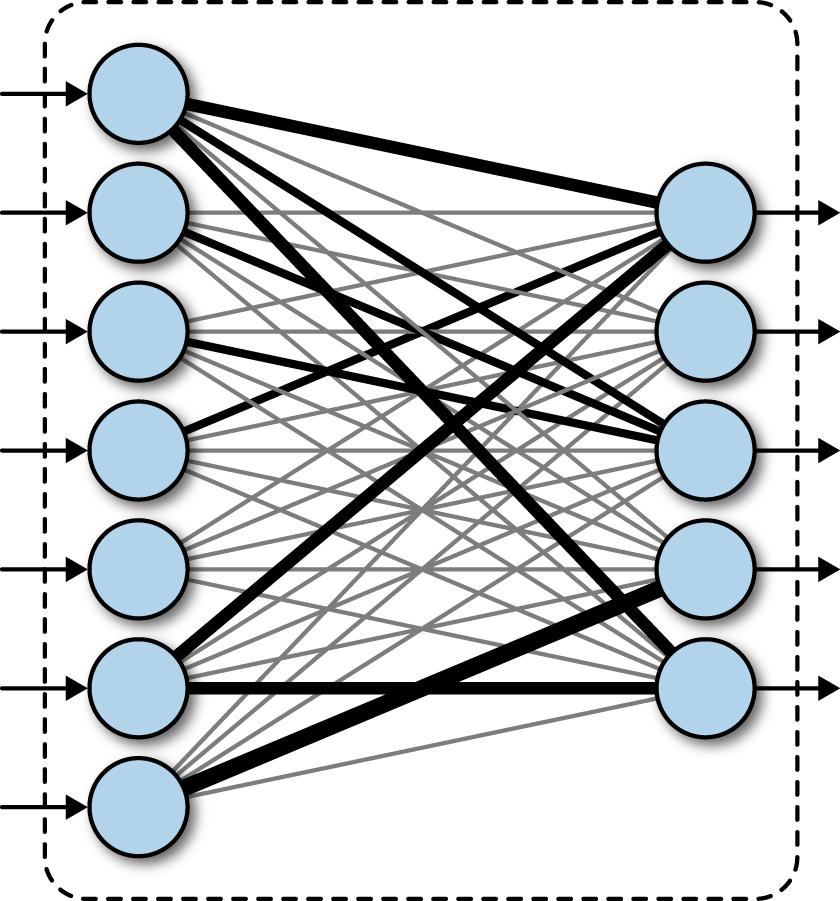
\includegraphics[height=7cm, width = 9cm]{img/fully_connected.png}
\caption{The illustration of fully connected layers. Each neuron is connected to all the neurons in the previous layer. From oreilly.com \label{fig_fc}}
\end{center}
\end{figure}

The fully connected layer can be implemented in Keras using the Dense layer API.
\begin{lstlisting}[language=python,frame=single]
keras.layers.Dense(units=1, activation='sigmoid', ...)
\end{lstlisting}
\subsubsection{Recurrent neural networks}
Another star of the deep learning algorithms is Recurrent Neural Networks (RNN). Recurrent neural networks are good at modeling sequential data. The input of an RNN is a sequence. Each chunk of the sequence is called a timestep. For example, in Fig. \ref{fig_RNN_timestep}, the network input is the sentence "What time is it". Each word or punctuation in the sentence is fed to a computation unit denoted by a circle. A single occurrence of the unit is called a timestep. RNN allows each hidden state to remember certain information from previous timesteps. The ability of carrying previous information makes RNN good at speech recognition, language translation, stock predictions etc. 
\begin{figure}[h!]
\begin{center}
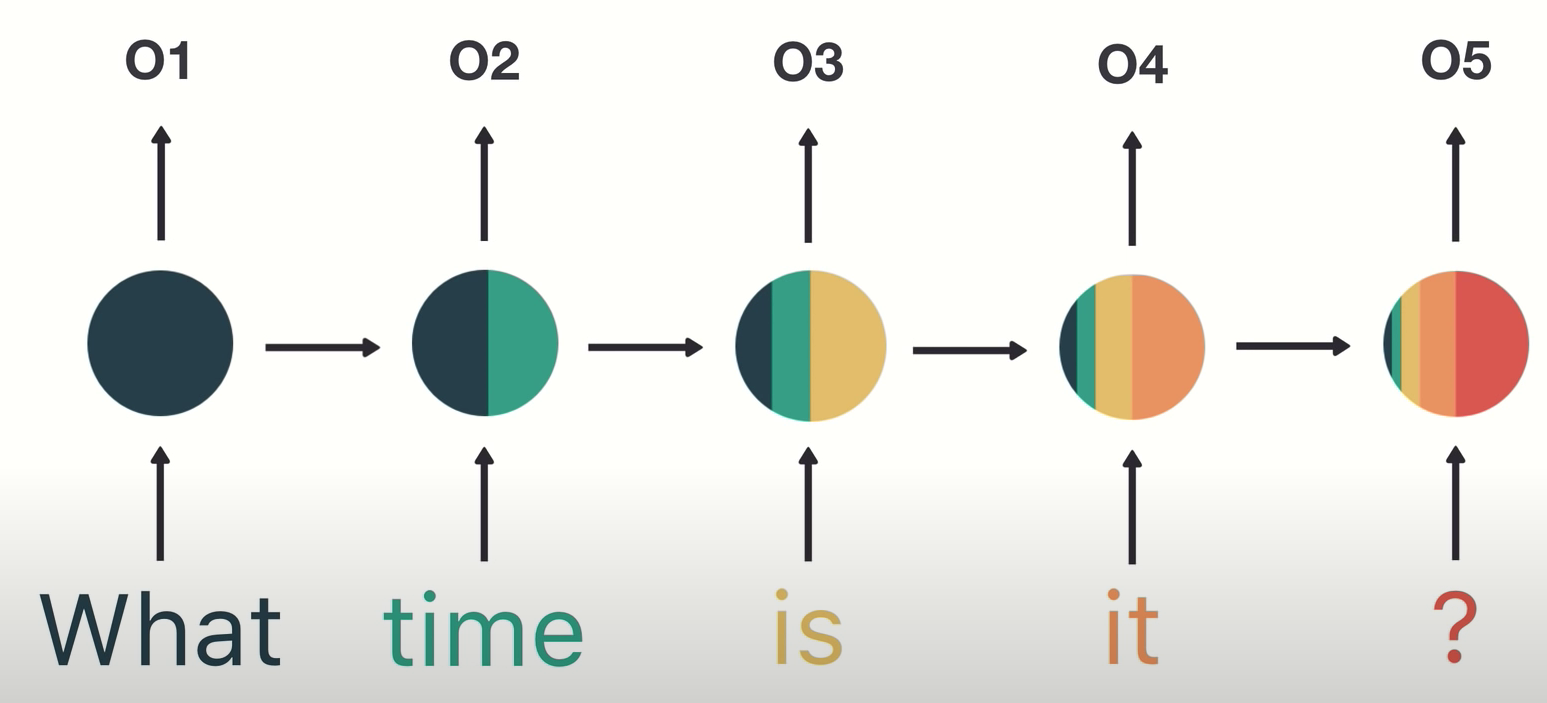
\includegraphics[width = 9cm]{img/RNN.png}
\caption{Time steps in a recurrent neural network. The network input is the sentence "What time is it?". Each word is fed to a unit in the RNN network. The occurrence of each unit is called a timestep. From towardsdatascience.com \label{fig_RNN_timestep}}
\end{center}
\end{figure}

 A single RNN cell is shown in Fig. \ref{fig_RNN}. Notice that the major difference between a RNN layer and a fully connected layer is that there are two inputs in each RNN cell, the input at the $t$th position $x^{<t>}$ and the output of the previous cell $a^{<t-1>}$. This way, the network manages to memories the information from previous sequences. $a^{<t-1>}$ and $x^{<t>}$ are multiply by their weights in the cell, and the weights are learned during training. 

\begin{figure}[h!]
\begin{center}
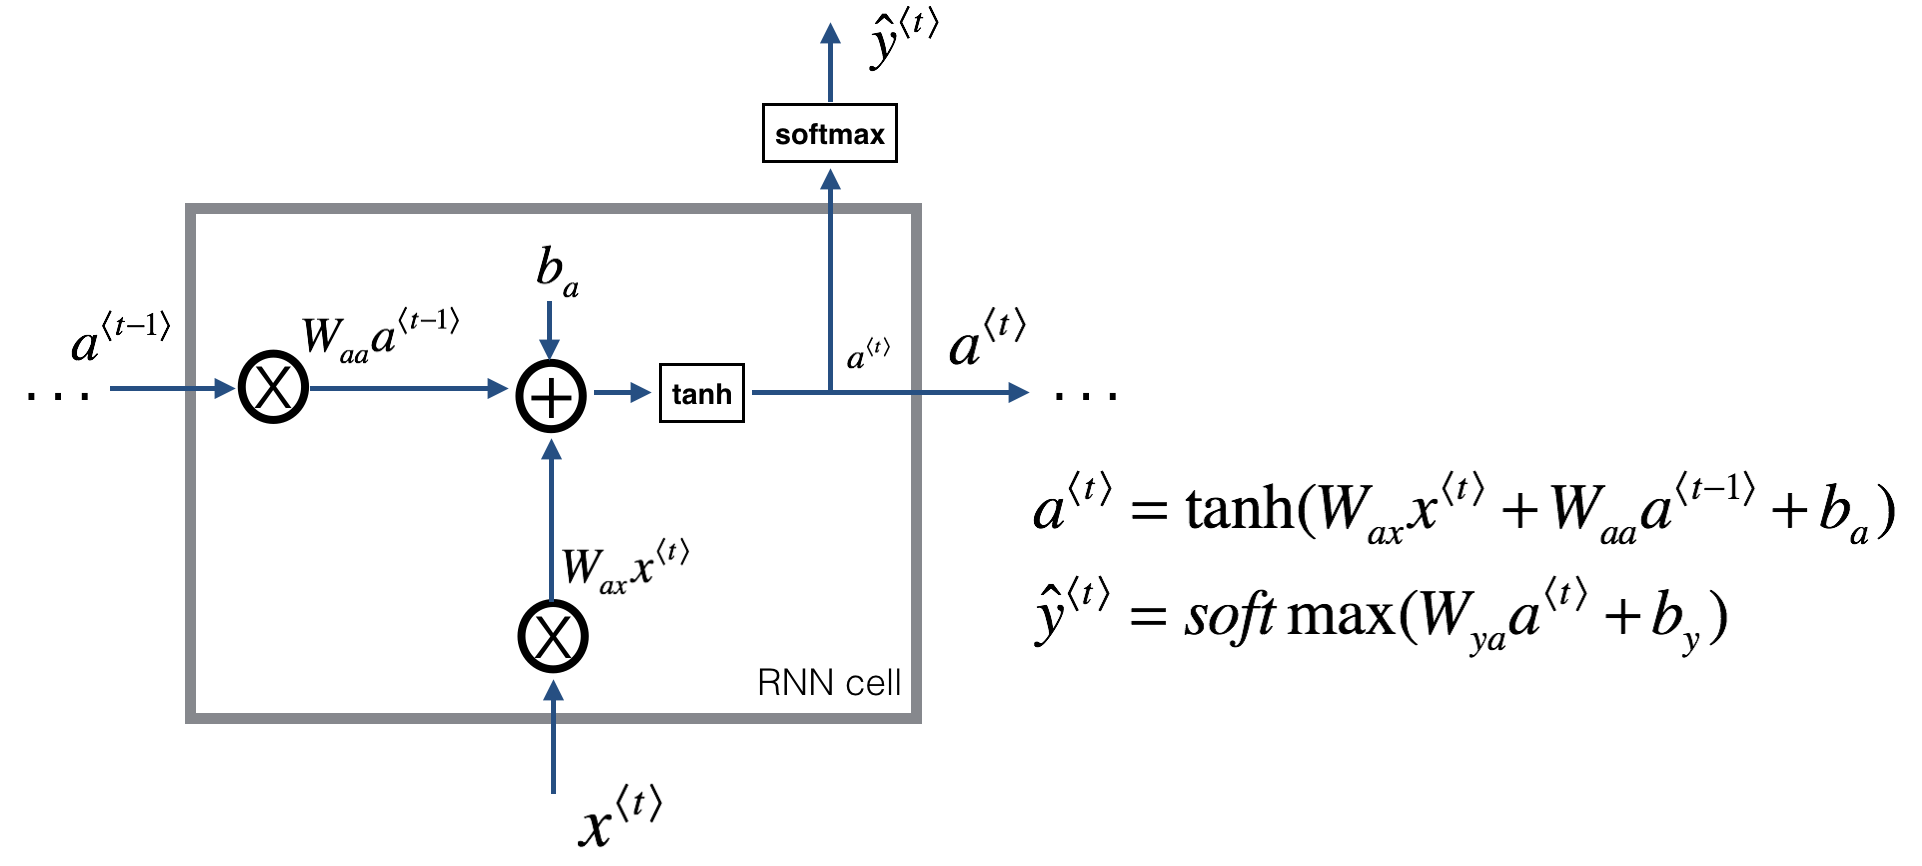
\includegraphics[width = 13cm]{img/basic_rnn.png}
\caption{A basic RNN cell. The inputs are: output from the previous unit $a^{<t-1>}$ and $t$th input $x^{<t>}$. From stanford.edu. \label{fig_RNN}}
\end{center}
\end{figure}

A major concern with the basic RNN is Vanishing Gradient \cite{pascanu2013difficulty} which is also called short term memory problem in RNN. When doing back propagation, each node in a layer calculates its gradient with respect to the effects of the gradients, in the layer before it. The adjustment is smaller and smaller through the chain rule. However, the importance of beginning part of input sequence could be dominant. For example, in the sentence "What time is it?", the words "what time" are very important even though it is at the beginning part of the sentence. Long short-term memory (LSTM) \cite{hochreiter1997long} and Gated Recurrent Unit \cite{cho2014learning} are developed to solve the Vanishing Gradient problem in RNN.

As shown in Fig. \ref{fig_LSTM_GRU}, LSTM and GRU cells are built based on the basic RNN cell. They are computationally more expensive than the basic RNN cell but able to maintain the information from the first time step till the last time step by introducing forget gates, input gates, output gates, cell state, update gates, reset gates. Gates contains an activation function that decides whether to remember or to forget the input value. LSTM and GRU have similar cell structure, and usually researchers empirically determine which one to use for a specific deep learning application.
\begin{figure}[h!]
\begin{center}
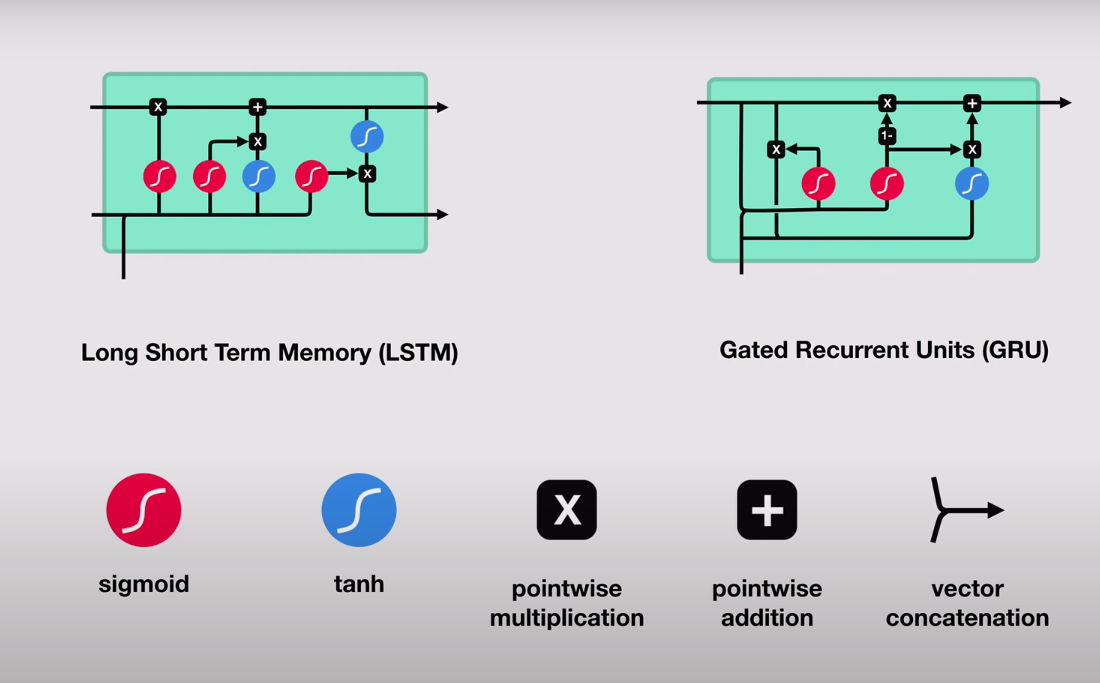
\includegraphics[width = 13cm]{img/LSTM_GRU.png}
\caption{A single LSTM and GRU unit. From towardsdatascience.com \label{fig_LSTM_GRU}}
\end{center}
\end{figure}

In Keras, LSTM, GRU can be implemented as follows.
\begin{lstlisting}[language=python,frame=single]
# LSTM
keras.layers.LSTM(units = 32, activation='tanh', ...)
# GRU
keras.layers.LSTM(units = 32, activation='tanh', ...)
\end{lstlisting}
\subsubsection{Ensemble networks}
Deep learning neural networks are nonlinear methods. This offers great flexibility in terms of fitting the training data, but a downside of this flexibility is that they are sensitive to the specifics of the training data and may find a set of weights each for a set of training data but does not apply to other data. This problem is called overfitting and often referred to as having a high variance \cite{goodfellow2016deep} as shown in Fig. \ref{fig_over_under_fitting}.
\begin{figure}[h!]
\begin{center}
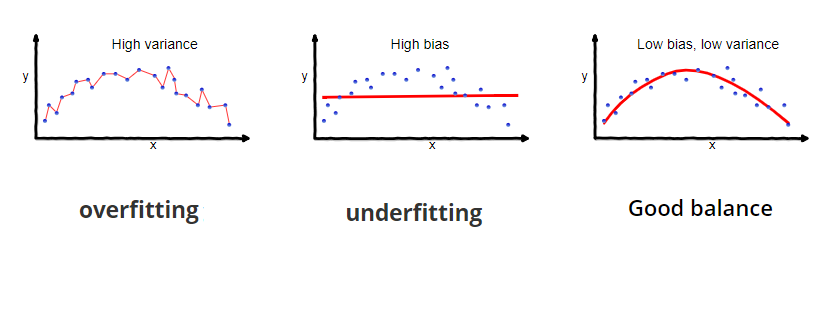
\includegraphics[width = 13cm]{img/over_under_fiting.png}
\caption{The illustration of overfitting, underfitting, and good balance. From towardsdatascience.com \label{fig_over_under_fitting}}
\end{center}
\end{figure}

One effective way of reducing the high variance is to train multiple models instead of a single model and then combine the predictions from all models, as shown in Fig. \ref{fig_ensemble_learning}. This is called ensemble learning.
\begin{figure}[h!]
\begin{center}
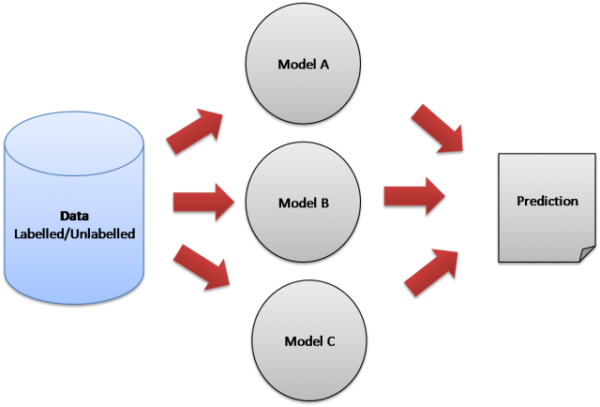
\includegraphics[width = 8cm]{img/ensemble_learning.png}
\caption{The illustration of ensemble learning. Three models A, B, and C are trained using the same training data, and the final prediction is the combination of the output from all three models. From towardsdatascience.com \label{fig_ensemble_learning}}
\end{center}
\end{figure}
\subsubsection{Dropout layers}
Ensemble learning can effectively reduce overfitting, but it is computationally more expensive as more models need to be trained. A single model can simulate the process of having different network architectures by dropping out nodes during training \cite{srivastava2014dropout}. As shown in Fig. \ref{fig_dropout}, the output of some nodes are randomly "dropped" to 0. This computationally cheap way is proven to be a remarkably effective regularization method to reduce overfitting. Dropout can be applied to all types of layers. In Keras, it is either integrated as a layer parameter or used directly as an independent layer. Below are some examples Keras dropout code.
\begin{lstlisting}[language=python,frame=single]
# 1. adding a dropout layer between two fully connected layers
keras.layers.Dense(units=64, ...)
keras.layers.Dropout(rate=0.5, ...)
keras.layers.Dense(units=1)
# 2. applying dropout in an LSTM layer
keras.layers.LSTM(units=32, dropout=0.5, ...)
\end{lstlisting}
\begin{figure}[h!]
\begin{center}
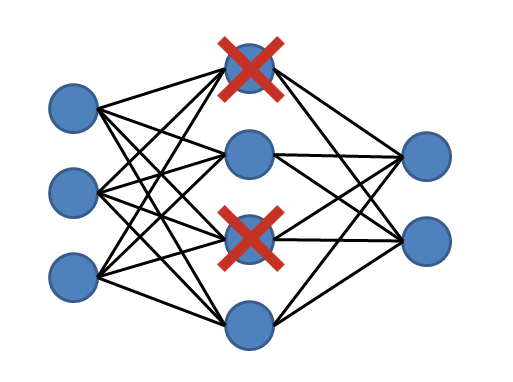
\includegraphics[height = 6cm, width = 10cm]{img/dropout.png}
\caption{An example of applying dropout in fully connected layers. During training, the two nodes in the middle layer are dropped out meaning that their outputs to the next layer become 0. \label{fig_dropout}}
\end{center}
\end{figure}
\subsubsection{Training, validation, and testing dataset}
Preparing the dataset is one of the most important steps in developing deep learning applications. Generally, in order to compare with other programs, the comparative performance on one or several gold standard testing datasets are needed. These testing datasets are often called benchmark data. One can easily train and overfit the benchmark and report good performance that fails to generalize to other datasets, so during the development process, the model should not be trained on the benchmark dataset or similar data. However, we still need a way is to tell if the model is trained well. The most popular way is to split the training dataset into two parts, training and validation. During the model development cycle, the model is trained on the training data. If the performance on the training data is satisfactory, the model is evaluated against the validation data. Results obtained on training and validation data should be similar, otherwise it is an indication of overfitting. This can be done for several rounds until the achievement of good performance. Then the performance on the testing data is reported. All adjustments to the model should be based on training and validation data only, not on benchmark data.
\subsubsection{Data augmentations and sampling}
As discussed earlier in Fig. \ref{fig_data_performance}, generally speaking, the more data to train a model, the better performance it renders. However, trainig data can be limited due to various reason. Many techniques are designed to synthetically create more data. This is called data augmentation. In computer vision, popular data augmentations include image mirroring, random cropping, and color shifting.  

Many machine learning algorithms are designed to train on classification data with balanced data, but biological data is often unbalanced. For example, in a tumor image classification dataset, most of the images are benign, and only a small portion is malignant. Data sampling is a collection of techniques that transform a training dataset in order to balance or better balance the class distribution \cite{chawla2004special}. Popular techniques include randomly under-sampling the majority class, randomly over-sampling the minority class, and Sythetic Minority Oversampling Technique (SMOT) \cite{chawla2002smote}.
\subsection{Previous Methods}
Similar to PPI predictions, the experimental methods for PPI binding sites identification are labor and time intensive. Computational methods are needed to bridge the gap, and many have been developed \cite{cao2006enhanced, ofran2007isis, du2009improved, chen2009sequence, london2010structural, chen2010sequence, murakami2010applying, xue2011homppi, amos2011binding, jones2012psicov, asadabadi2013predictions, singh2014springs, wang2014fast, geng2015prediction, laine2015local, hwang2016hybrid, maheshwari2015prediction, liu2016prediction, wei2016protein, maheshwari2016template, jia2016ippbs, zhang2019sequence, wang2019protein, zhang2019scriber, zeng2019protein, xie2020prediction}. Out of the above mentioned twenty six computational methods, all but one are machine learning based. Computational methods can be classified into three categories, sequenced based, structure based, and combined. Among them, sequence-based approaches are usually faster and cheaper. They are also more universal because comparing to sequence information, structure information is still limited. 

Machine learning methods use feature groups to represent each protein sequence. Widely used features such as position-specific scoring matrix (PSSM), evolutionary conservation (ECO), putative relative solvent accessibility (RSA) have been assessed in \cite{zhang2019comprehensive}. High-scoring segment pair (HSP) has been used in previous methods for PPI prediction \cite{li2017sprint}. One-hot vectors \cite{zhang2019sequence, zeng2019protein} and amino acid embedding \cite{asgari2015continuous, heinzinger2019modeling, asgari2019probabilistic} have also been empirically explored to represent protein sequences.

The learning structure is crucial to PPI binding sites classification problems. Previously explored architectures include random forest \cite{wei2016protein, wang2019protein}, SVM \cite{wei2016protein}, logistic regression \cite{zhang2019scriber}, Bayes classifier \cite{murakami2010applying}, artificial neural networks \cite{singh2014springs}. Recently, convolutional neural network (CNN) \cite{zeng2019protein} and recurrent neural network (RNN) \cite{zhang2019sequence} have also been applied to solve this problem. 

\subsubsection{PIPE-sites}
PIPE-Sites \cite{amos2011binding} is a algorithmic based PPI binding site program based on the PPI prediction program PIPE \cite{pitre2006pipe}. It requires only protein sequences and known interactions. As one of the few partner-specific sites predictors, PIPE-Sites is able to predict different binding sites for the same protein but with different partners. For example, protein A interacts with protein B and C, and the binding sites between A-B and A-C are different. PIPE-sites is able to predict these different sites in protein A.

The algorithm of PIPE-Sites is shown using an example in Figure \ref{fig_PIPE-Sites}. Using the PIPE program, the scoring matrix is built for a protein pair, the program first finds the peak location. Then it extend from the peak towards all four directions until the value drops below a predefined threshold, percentPeak. Residues within the window are considered binding sites. If there are multiple peaks, PIPE-sites will generate a ranked list, in descending order, of potential binding sites.

\begin{figure}[h!]
\begin{center}
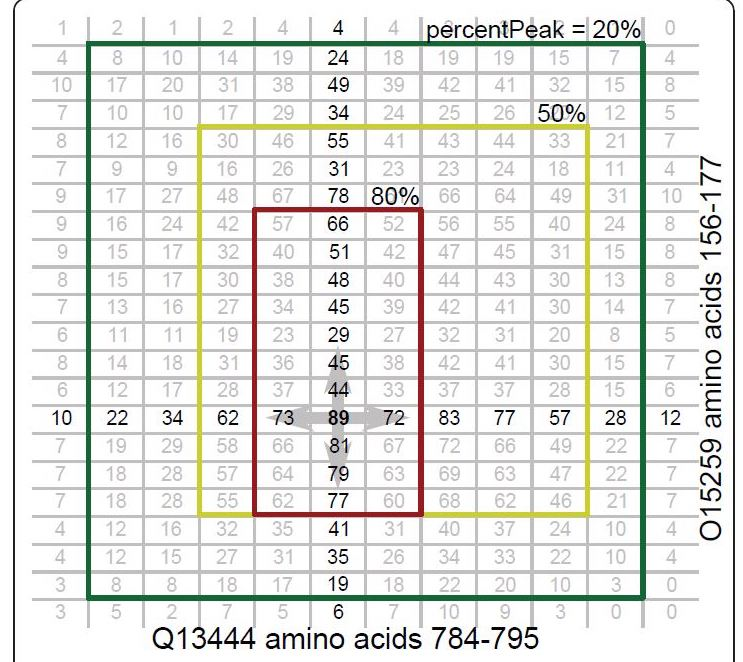
\includegraphics[height =9 cm]{img/PIPE_site_cut.JPG}
\caption{The walk algorithm of PIPE-Sites. PIPE-Sites detects first the peak in the matrix 89. Then it extends towards all four directions until the score drops below a threshold percentPeak. Depends on the choice of percentPeak, different windows are drawn. Residues within the window are considered binding sites. From: \cite{amos2011binding}  \label{fig_PIPE-Sites}}
\end{center}
\end{figure} 

% In the paper of PIPE-sites \cite{amos2011binding}, the authors claim that PIPE-sites is accurate by checking the predicted sites against some domain databases. Figure \ref{fig_PIPE-Sites_eg} shows examples of two matrices that PIPE produces. The left one shows a highly possible binding site between protein Q13444 and protein O15259. The peak location is the predicted site (location 700-800 in Q13444, location 100-200 in O15259). The right picture indicates that there is no interaction between YGL055W and YBL090W as there is no high peak in the matrix. 
% \begin{figure}[h!]
% \begin{center}
% 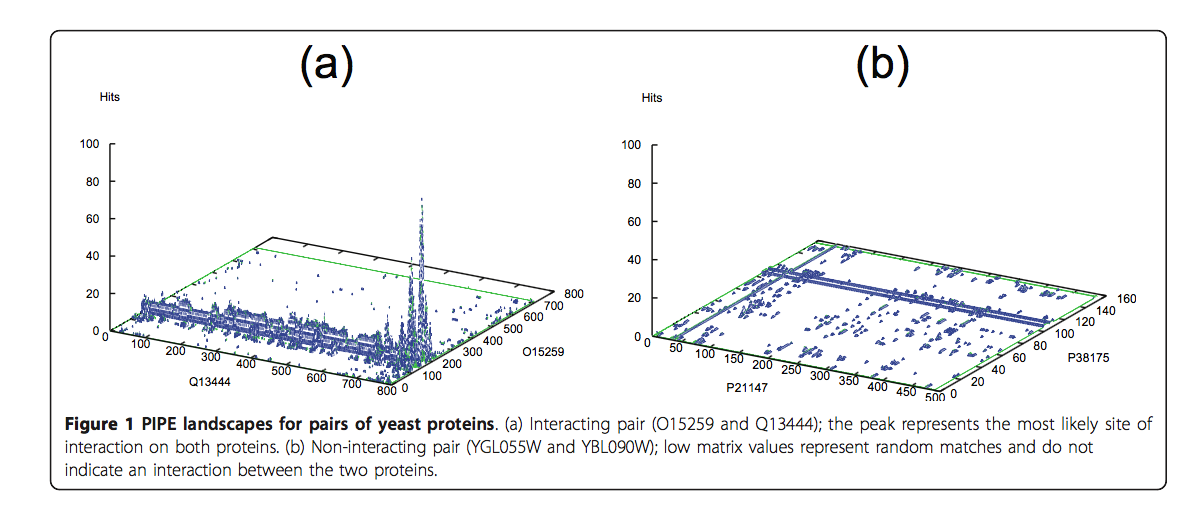
\includegraphics[height = 6 cm]{img/pipe_sites_ex.png}
% \caption{Examples of PIPE-Sites matrices. (From: \cite{amos2011binding})  \label{fig_PIPE-Sites_eg}}
% \end{center}
% \end{figure} 

\subsubsection{DLPred}
DLPred \cite{zhang2019sequence} is a sequence based protein binding predictor published in 2019. Its architecture is shown in Fig. \ref{fig_DLPred}. The main layers in DLPred model are simplified LSTM layers and fully connected layers. The simplified LSTM is developed by the authors, and the main purpose is to reduce the time consumption. The features used are PSSM, physical properties, hydropathy index, physicochemical characteristics, PKx (the negative of the logarithm of the dissociation con- stant for any other group in the molecule), conservation score, and one-hot encoding for protein sequences. DLPred also adopts a filtered sampling technique such that sequences with more binding residue are picked. They empirically show that this helps deal with the imbalance of the protein biding problem.
\begin{figure}[h!]
\begin{center}
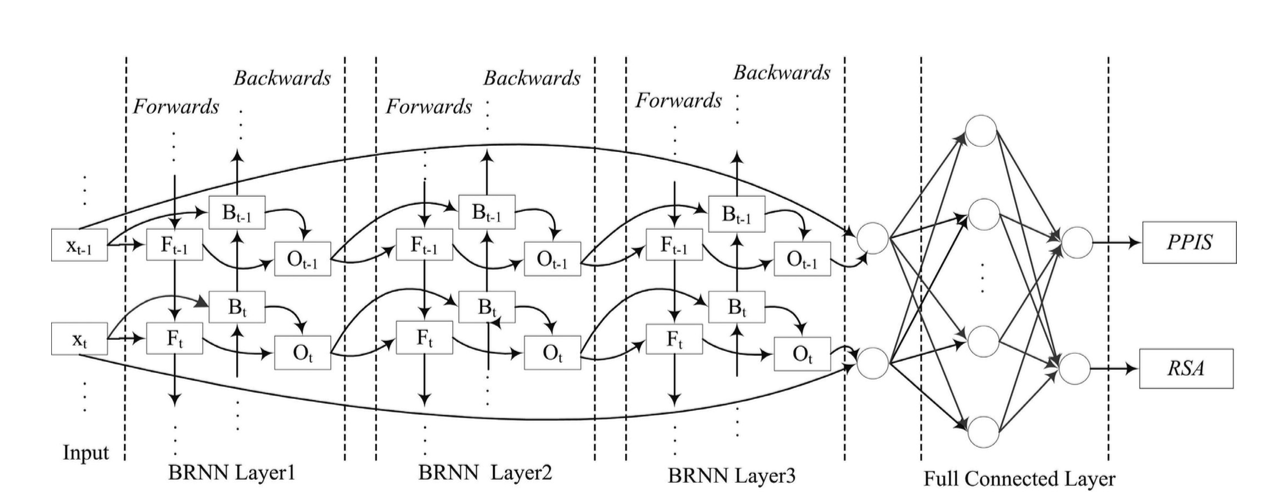
\includegraphics[height = 6 cm]{img/DLPred.png}
\caption{The architecture of DLPred. Three BSLSTM layers are followed by two fully connected layers with highway connection.  (From: \cite{zhang2019sequence})  \label{fig_DLPred}}
\end{center}
\end{figure} 

\subsubsection{DeepPPISP}
DeepPPISP \cite{zeng2019protein} is a recent protein binding prediction utilizing secondary structure. As shown in Fig. \ref{fig_DeepPPISP}, the network structure of DeepPPISP consists of a TextCNN component to extract feature features and two fully connected layers to classify protein binding residue. The TextCNN is a variation of the convolution layers meant to handle lower dimension tensor. DeepPPISP is highlighted for the usage of both local and global information. For each given amino acid, the local information is the neighboring seven amino acids of the target amino acid, and the global information is its     neighboring 500 amino acids. It is shown empirically in the paper that the usage of global information largely helps the prediction. 
\begin{figure}[h!]
\begin{center}
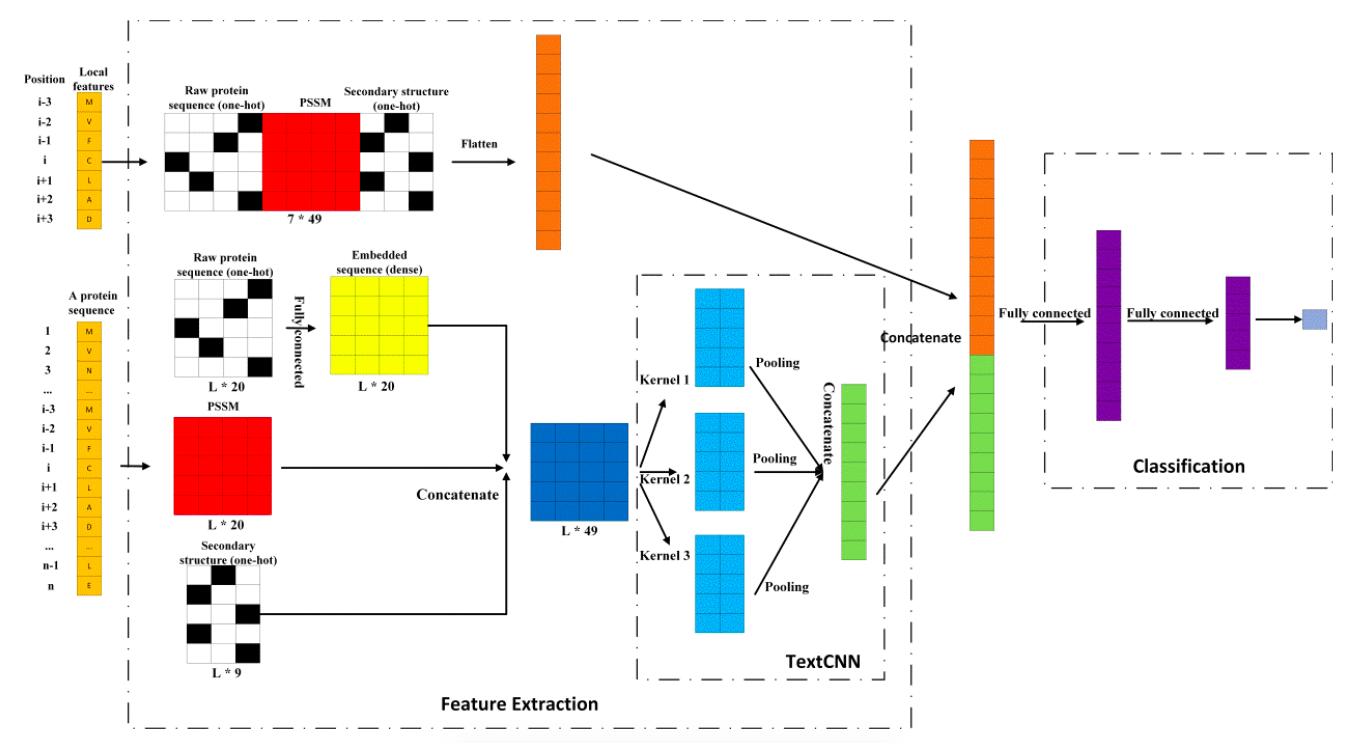
\includegraphics[width = 14cm]{img/DeepPPISP.png}
\caption{The architecture of DeepPPISP. The inputs are both sub-sequence (local) and whole protein sequence. For local features, sequence embedding, PSSM, and secondary structure are combined and then flattened a local feature vector. For global features, sequence embedding, PSSM, and secondary structure are concatenated and then passed through TextCNN layers. The features extracted from local and global sequence are further concatenated and passed through fully connected layers.  (From: \cite{zeng2019protein})  \label{fig_DeepPPISP}}
\end{center}
\end{figure} 

\subsubsection{SCRIBER}
SCRIBER \cite{zhang2019scriber} is another sequence-based protein binding residue predictor published in 2019. It uses the following feature: putative relative solvent accessibility (RSA), evolutionary conservation (ECO), relative amino acid propensity (RAAP) for binding, and the selected relevant physiochemical properties, putative protein binding intrinsically disordered regions, putative secondary structure (SS), and selected physicochemical properties of amino acids (aliphaticity, aromaticity, acidity and size). The core layer of the model is a simple logistic regression. The key innovative idea of SCRIBER is that it is trained using not only protein-protein binding information, but also protein binding information with RNA, DNA, ligand, and other type. As shown in Fig. \ref{fig_SCRIBER}, in the first layer of SCRIBER, five different models are trained using five binding information. In the second layer, the prediction values of the five models are used as input to train another model aiming to predict protein-protein binding sites only. The intuition is that models make false predictions because they mistakenly cross-predict other types of binding. For example, a non-protein-protein binding residue is predicted to have high propensity for protein-protein binding, but it is actually a residue for DNA binding. The mistake happens because of the different types of bindings share some similar properties. Because SCRIBER is not a deep learning based method, it uses a relatively small training dataset containing 843 proteins.
\begin{figure}[h!]
\begin{center}
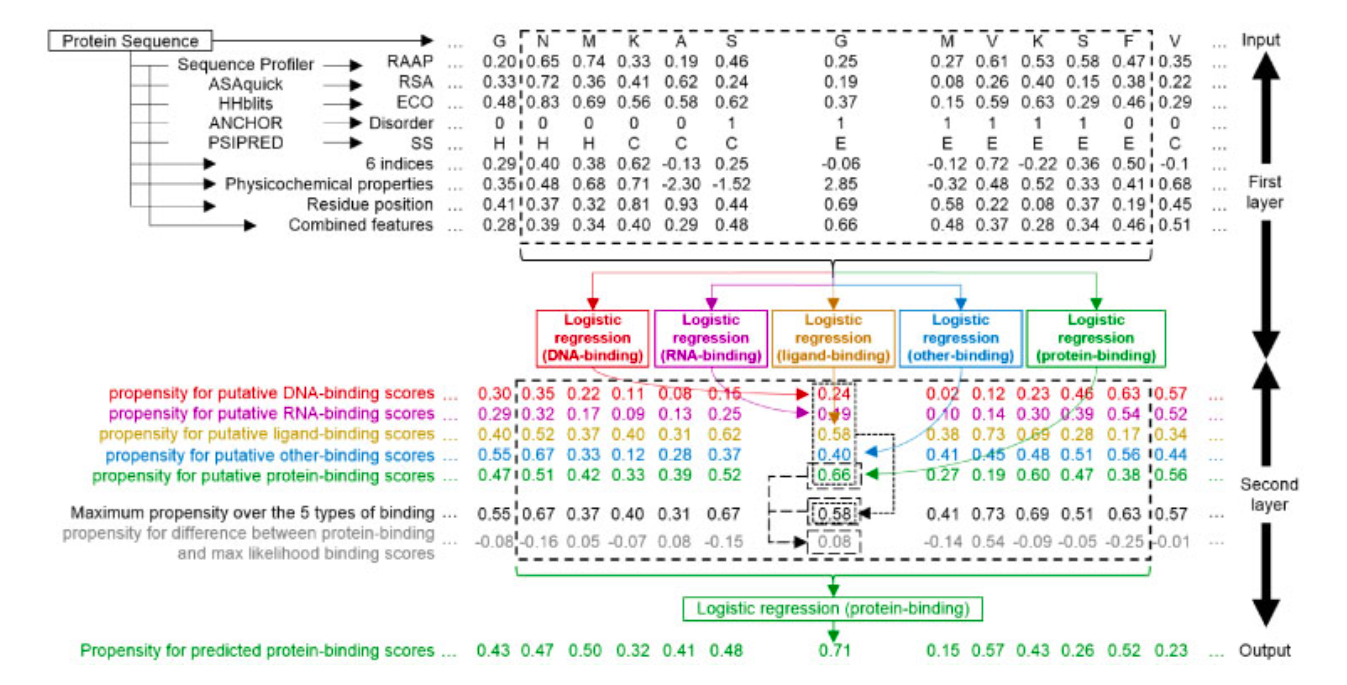
\includegraphics[height = 7cm]{img/SCRIBER.png}
\caption{The architecture of SCRIBER. The first layer predicts the propensities for DNA-binding (red), RNA-binding (violet), small ligand-binding (orange), other-binding (blue) and protein-binding (green) residues. These propensities are used together in the second layer to predict protein-protein binding sites. (From: \cite{zhang2019scriber})  \label{fig_SCRIBER}}
\end{center}
\end{figure} 
\section{Methods}
This section describes in details our program DELPHI for binding site prediction. It is trained on a big dataset comparing to the competitors. DELPHI combines a CNN and a RNN components with a many-to-one structure. It uses twelve features to represent protein sequences, among them three are used first time for site prediction. The comparative analysis shows that DELPHI has a better prediction accuracy in all evaluation metrics. 

\subsection{Training Data Preparation}
Training data is one of the most important factors in training a model. An trend in applied machine learning research field is that a good publication always comes good data. 
    
\subsubsection{Raw data}
We first collected a relatively large amount of raw data. A high quality dataset was provided in \cite{zhang2019comprehensive}, where proteins were solved structurally in complex from the BioLiP \cite{yang2012biolip} database. In BioLip, two residue are considered binding if the distance between the atoms of the 
two residues $<$0.5+sum of the Van der Waal's radii of the two atoms. BioLip IDs are then mapped into UniProt IDs using SIFTS \cite{velankar2012sifts} to insure we work with complete sequences. Then we left with sequences annotated with Protein, DNA, RNA, and small ligands binding information at the residue level. We kept only the sequences with protein-protein binding information to focus on protein-protein binding.
\subsubsection{Similarities eliminations}
We further processed this dataset by eliminating similarities. We removed any sequences from training dataset sharing more than 25\% similarities, as measured by PSI-CD-hit \cite{li2006cd,fu2012cd}, with any sequences in testing datasets. It is well acknowledged that similar sequences between training and testing datasets negatively affect the generalization of the evaluated performance of a machine learning model. Also, proteins with higher levels of similarity can be accurately predicted by the alignment-based methods \cite{zhang2018review}. The similarity threshold is picked differently by different programs ranging from 25\% to 50\%. We picked the strictest value of 25\% to match to one of the closest competing programs, SCRIBER \cite{zhang2019scriber}, for a fair comparison. We used PSI-CD-HIT because it is fast, accurate and well maintained in the CD-HIT suite. Also, it is able to cluster sequences with similarity at low as 25\%, whereas CD-HIT works only down to 40\%. Finally, we ran PSI-CD-hit again on the rest of the training protein sequences so no sequences shared more than 25\% similarities among training data. This ensures the training data is as diverse as possible. The commands to cluster proteins using PSI-CD-HIT are as follows.
\begin{lstlisting}[language=bash,frame=single]
# convert fasta file to blast database format
$ makeblastdb -in [fasta_file_name] -dbtype prot
# compute protein clusters
$ psi-cd-hit/psi-cd-hit.pl -i [fasta_file_name] -o [out_file_name] -c 0.25
\end{lstlisting}
\subsubsection{Data split}
After the similarities elimination process, A dataset of 9,982 protein sequences was constructed. From it, we randomly pick eight ninth (8,872) as the training dataset and one ninth (1,110) as the validation dataset. This can be done by using the model\_selection module from sklearn. The commands are as follows.
\begin{lstlisting}[language=python,frame=single]
kfold = KFold(n_splits=9)
for train, test in kfold.split(dataset_all)
    ...
\end{lstlisting}


\subsection{Features}
DELPHI uses 12 features groups, shown in Table \ref{tab_feture}, including high-scoring segment pair (HSP), a variation of 3-mer amino acid embedding (ProtVec1D), position information, position-specific scoring matrix (PSSM), evolutionary conservation (ECO), putative relative solvent accessibility (RSA), relative amino acid propensity (RAA), putative protein-binding disorder, hydropathy index, physicochemical characteristics, physical properties, and PKx. Each input is represented by a 39 dimensional feature vector profile. To the best of our knowledge, this study is the first time that HSP, ProtVec1D, and position information are being used in binding sites classification problems. The computation of each of these two new features is described next.

\begin{table}[htbp]
  \centering
  \caption{The feature groups used by DELPHI. The first column indicates the name of each feature. The second column describes the program used to obtain the feature. ``Load'' means the value for a specific amino acid is known from previous work, and it is loaded in the DELPHI program. ``Compute'' means DELPHI performs additional computation to that feature. The last column shows the dimension of each feature group. Full details are given in the text.}
    \begin{tabular}{p{20.93em}p{11em}r}
    \toprule
    Feature & Program & \multicolumn{1}{p{5.145em}}{Dimension} \\
    \midrule
    High-scoring segment pair (HSP) & SPRINT and compute & 1 \\
    % \midrule
    3-mer amino acid embedding (ProtVec1D) & Load and compute & 1 \\
    % \midrule
    Position information & Compute & 1 \\
    Position-specific scoring matrix (PSSM) & Psi-Blast & 20 \\
    % \midrule
    Evolutionary conservation (ECO) & Hhblits & 1 \\
    % \midrule
    Putative relative solvent accessibility (RSA) & ASAquick & 1 \\
    % \midrule
    Relative amino acid propensity (RAA) & Load  & 1 \\
    % \midrule
    Putative protein-binding disorder & ANCHOR & 1 \\
    % \midrule
    Hydropathy index & Load  & 1 \\
    % \midrule
    Physicochemical characteristics & Load  & 3 \\
    % \midrule
    Physical properties & Load  & 7 \\
    % \midrule
    PKx   & Load  & 1 \\
    \bottomrule
    \end{tabular}%
  \label{tab_feture}%
\end{table}%

High-scoring segment pair (HSP): An HSP is a pair of similar sub-sequences between two proteins. The similarities between two sub-sequence of the same length are measured by scoring matrices such as PAM and BLOSUM. SPRINT \cite{li2017sprint} is used for computing all HSPs as it detects similarities fast and accurately among all proteins in training and testing. After obtaining the HSPs, the score for the $i$th residue, $P[i]$, of a testing protein $P$, denoted $\text{HSP}_{\text{score}}(P[i])$, is calculated as follows. Assume we have an HSP, $(u,v)$, between $P$ and a training protein $Q$ such that $u$ covers the residue $P[i]$, that is, position $i$ in $P$ is within the range covered by $u$. Let $j$ be the position in $Q$ that corresponds to $i$, that is, the distance in $P$ from the beginning of $u$ to $i$ is the same as the distance in $Q$ from the beginning of $v$ to $j$. If $Q[j]$ is a known interacting residue, then we add the PAM120 score between $P[i]$ and $Q[j]$ to the HSP score of $P[i]$:
\[
\text{HSP}_{\text{score}}(P[i]) = \!\!\!\!\!\!\sum_{\stackrel{\text{\tiny HSPs covering $P[i]$}}{\text{\tiny $Q[j]$ interacting residue}}}\!\!\!\!\!\! \max(0, \text{PAM120}(P[i], Q[j])) \ .
\]
The 3-mer amino acid embedding (ProtVec1D): We developed this feature based on ProtVec \cite{asgari2015continuous}. ProtVec uses word2vec \cite{mikolov2013distributed} to construct a one hundred dimensional embedding for each amino acid 3-mer. It is shown in \cite{asgari2015continuous} that ProtVec can be applied to problems such as protein family classification, protein visualization, structure prediction, disordered protein identification, and protein-protein interaction prediction. Since using the ProtVec embedding in our program slows down significantly the deep learning model, especially during training, we replaced the one hundred dimensional vector by one dimensional value, which is the sum of the one hundred components; we call this ProtVec1D. According to our tests, ProtVec1D achieves, in connection with the other feaures, the same prediction performance as ProtVec. In Keras, a pre-trained embedding layer can be use as follows.
\begin{lstlisting}[language=python,frame=single]
# initialize the pre-trained embedding as a dictionary
embedding_matrix = {}
...
# add an embedding layer with pre-traind weights
keras.layers.Embedding(input_dim = 31, output_dim = 100,
weights=[embedding_matrix], trainable=False)
\end{lstlisting}

Position information: In natural language processing tasks, position information is shown useful. The popular network Bert \cite{devlin2018bert} utilizes this information to guide its translation process. It is also shown by DeepPPISP \cite{zeng2019protein} that the global information of a protein helps the prediction of interfaces. Inspired by the two networks, we use the position information of each amino acid as an input feature hoping that it provides certain global information of a protein. The position of an amino acid in a protein is in the range of 1 to the length of the protein. Then the position is divided by protein's length so that the value is between 0 to 1.

Position-specific scoring matrix (PSSM): PSSM matrices are widely used in protein interaction related problems. They contain the evolutionary conservation of each amino acid position by aligning an input sequence with protein databases. The PSSM matrices are computed using PSI-Blast \cite{altschul1997gapped} with the expectation value (E-value) set to 0.001 and the number of iterations set to 3. PSI-Blast performs multiple alignment on each input sequence against the non-redundant database. PSSMs take fairly a long time to compute, but for each sequence, it only needs to be done once. The psiblast command I used is as follows.
\begin{lstlisting}[language=bash,frame=single]
$ psiblast -query [input_protein_fasta] -db [nr] -num_threads 3
-out_ascii_pssm ${out_pssm} -num_iterations 3
\end{lstlisting}

Evolutionary conservation (ECO): ECO also contains evolutionary conservation, but in a more compact way. To compute the ECO score, the faster multiple alignment tool HHBlits \cite{remmert2012hhblits} is run against the non-redundant Uniprot20 database with default parameters. The one dimensional conservation value is computed using the formula described in \cite{zhang2019comprehensive}. The commands used for conducting multiple alignment using hhblits as follows.
\begin{lstlisting}[language=bash,frame=single]
$ hhblits -i [input] -ohhm [output]  -d [database] -hide_cons 
-hide_pred -hide_dssp -v 0  -neffmax 1 -n 1
-out_ascii_pssm ${out_pssm} -num_iterations 3
\end{lstlisting}

Putative relative solvent accessibility (RSA): The solvent accessibility is predicted using ASAquick \cite{faraggi2014accurate}. The values are obtained in the from rasaq.pred file in each output directory. The ASAquick command is as follows.
\begin{lstlisting}[language=bash,frame=single]
$ ASAquick [input]
\end{lstlisting}


Relative amino acid propensity (RAA): The AA propensity for binding is quantified as relative difference in abundance of a given amino acid type between binding residues and the corresponding non-binding residues located on the protein surface. The RAA for each amino acid type is computed in \cite{zhang2019comprehensive} by using the program of  \cite{vacic2007composition}.

Putative protein-binding disorder: The putative protein-binding disorder is computed using the ANCHOR program \cite{dosztanyi2009anchor}. The used ANCHOR command is as follows.
\begin{lstlisting}[language=bash,frame=single]
$ anchor [input] -d [ANCHOR_DIR]  > ${raw_Anchor_dir}/${f_basename}.anchor
\end{lstlisting}

Hydropathy index: Hydrophobicity scales is experimentally determined transfer free energies for each amino acid. It contains energetics information of protein-bilayer interactions \cite{wimley1996experimentally}. The values are computed in \cite{kyte1982simple}.

Physicochemical characteristics: For each protein, this includes three features: the number of atoms, electrostatic charges and potential hydrogen bonds for each amino acid. They are taken from \cite{zhang2019sequence}.

Physical properties: We use a 7-dimensional property of each amino acid type. They are a steric parameter (graph-shape index), polarizability, volume (normalized van der Waals volume), hydrophobicity, isoelectric point, helix probability and sheet probability. The pre-computed values are taken from \cite{zhang2019sequence}.

PKx: This is the negative of the logarithm of the dissociation constant for any other group in the molecule. The values for each amino acid type is taken from \cite{zhang2019sequence}.

After computing all the feature vectors, the values in in each row vector are normalized to a number between 0 to 1 using formula (\ref{eq_normalized}) where \textit{v} is the original feature value, and max and min are the biggest and smallest value observed in the training dataset, resp. This is to ensure each feature group are of the same numeric scale and help the model converge better:

\begin{equation}
v_\text{norm}=\dfrac{v-\text{min}}{\text{max}-\text{min}}\label{eq_normalized}
\end{equation}

\subsection{Model Architecture}
\subsubsection{Architecture overview}
DELPHI has an architecture that is inspired by ensemble learning. The intuition of the design is that different components of the model capture different information, and another deep neural network is trained to only select the most useful ones. As shown in Fig. \ref{fig_architecture}, the model consists of three parts, a convolutional neural network (CNN) component, an recurrent neural network (RNN) component, and an ensemble component. The core layers of the CNN and RNN components are convolution and bidirectional gated recurrent units (GRU) layers. The ensemble model decodes the output of the first two components.  

\begin{figure*}
\centering
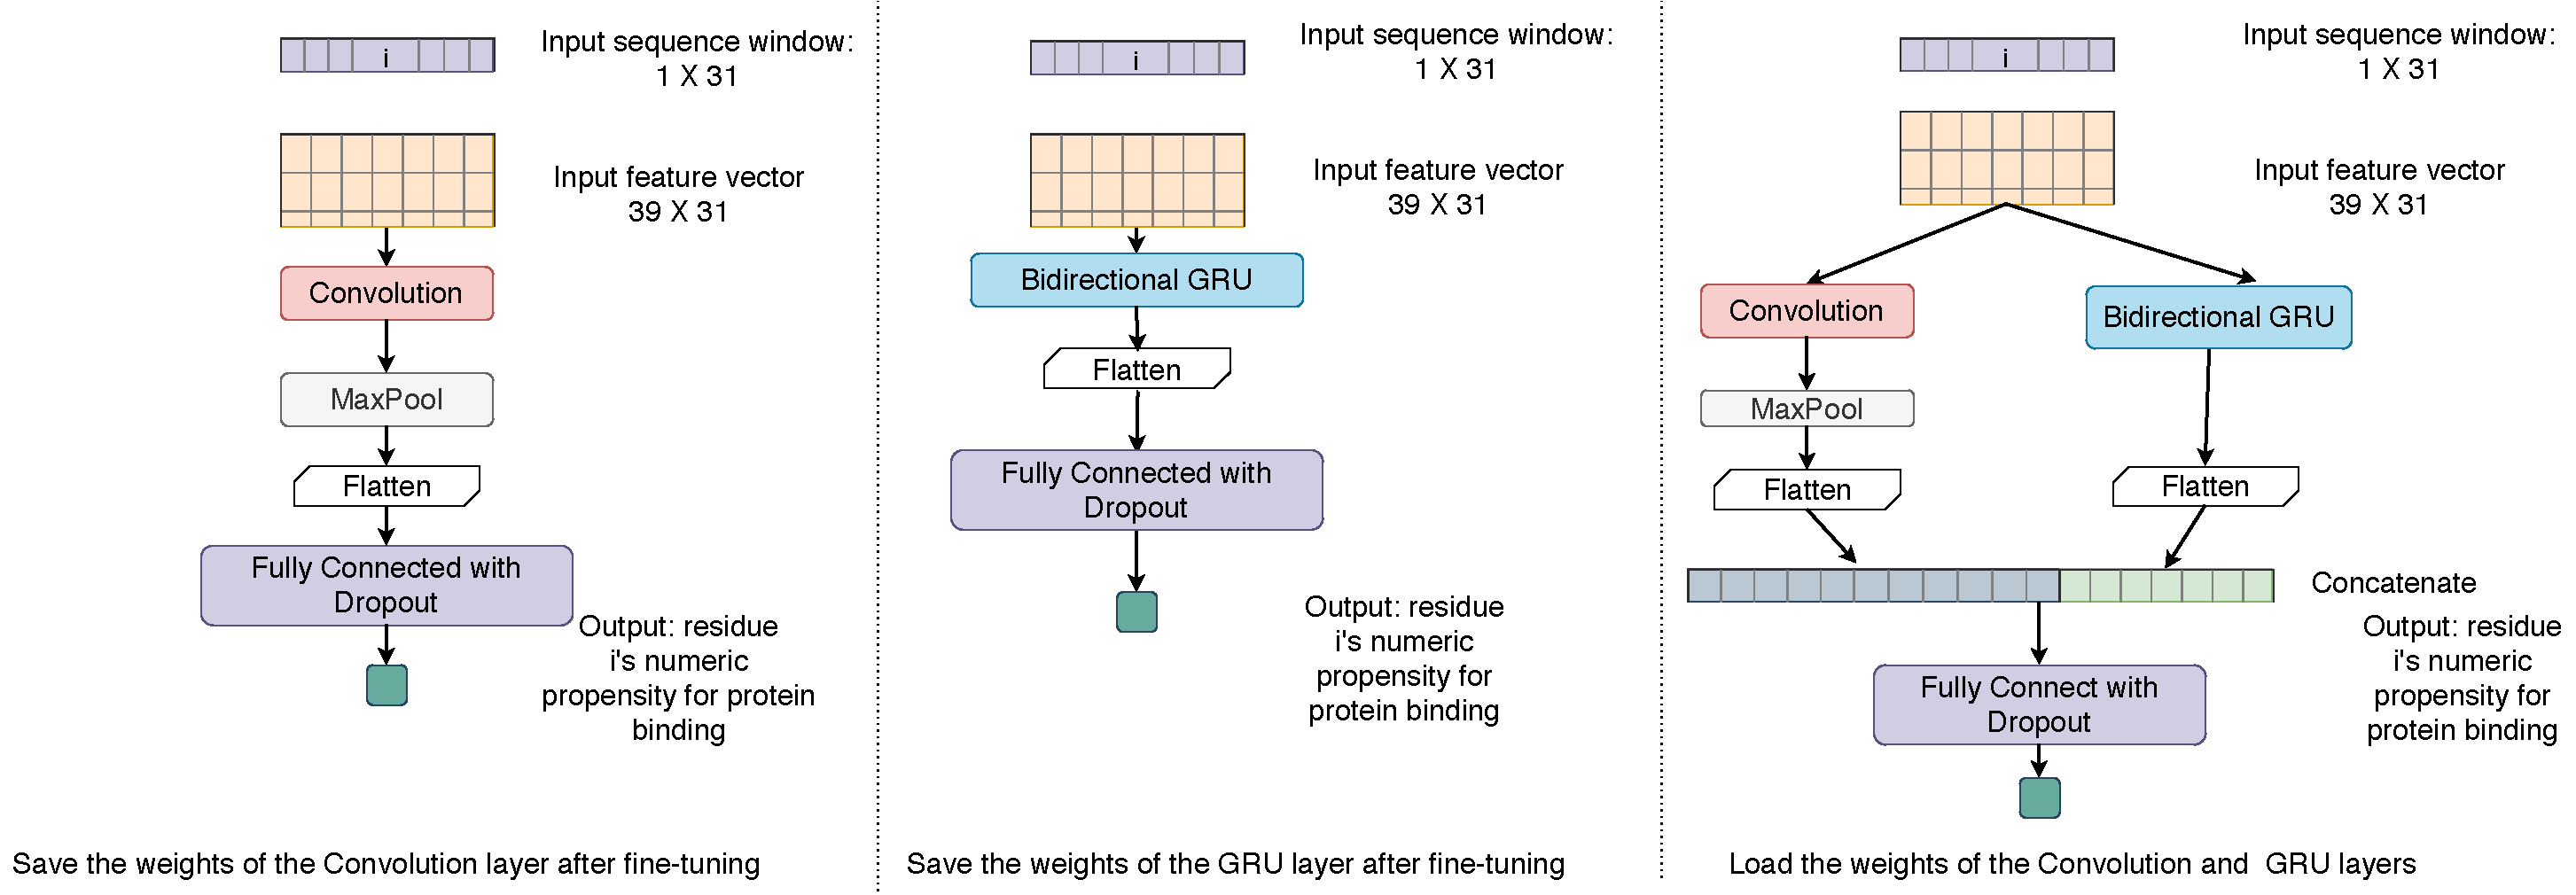
\includegraphics[width=\textwidth]{img/Model_architecture.pdf}
\caption{The architecture of DELPHI. Left: the CNN component of the model. Middle: the RNN component of the model. Right: The ensemble model. 
  \label{fig_architecture}}
\end{figure*}
\subsubsection{Many-to-one structure}
Another very useful characteristic of the model is its many-to-one structure, meaning that the information of many residues are used to prediction the binding propensity of the centered single residue. As illustrated in Fig. \ref{fig_many2one}, for each amino acid as the prediction target, a window of size 31, centred on the amino acid position, is used to collect information from the neighbouring 30 residues to help the prediction. A sliding window is used to capture each 31-mer. The size 31 is determined experimentally. The beginning and the ending part of the sequence are padded with zeros. The many-to-one structure has two advantages. Firstly, it serves as a data augmentation technique. Deep learning models need large amount of data to train, and comparing to image classifiers, models in proteomics have access to orders of magnitude less data. Using each residue multiple times during the training process helps the model learn better. Secondly, it makes the model more robust. The lengths of protein sequence vary from less than one hundred to several thousand, and most a many-to-many models have a fixed input length of near 500. During training, sequences around length 500 are often picked. However, during testing, input sequences are random and need to be either padded or cut into pieces. The different average lengths between training and testing could potentially make the model less general. 
\begin{figure*}
\centering
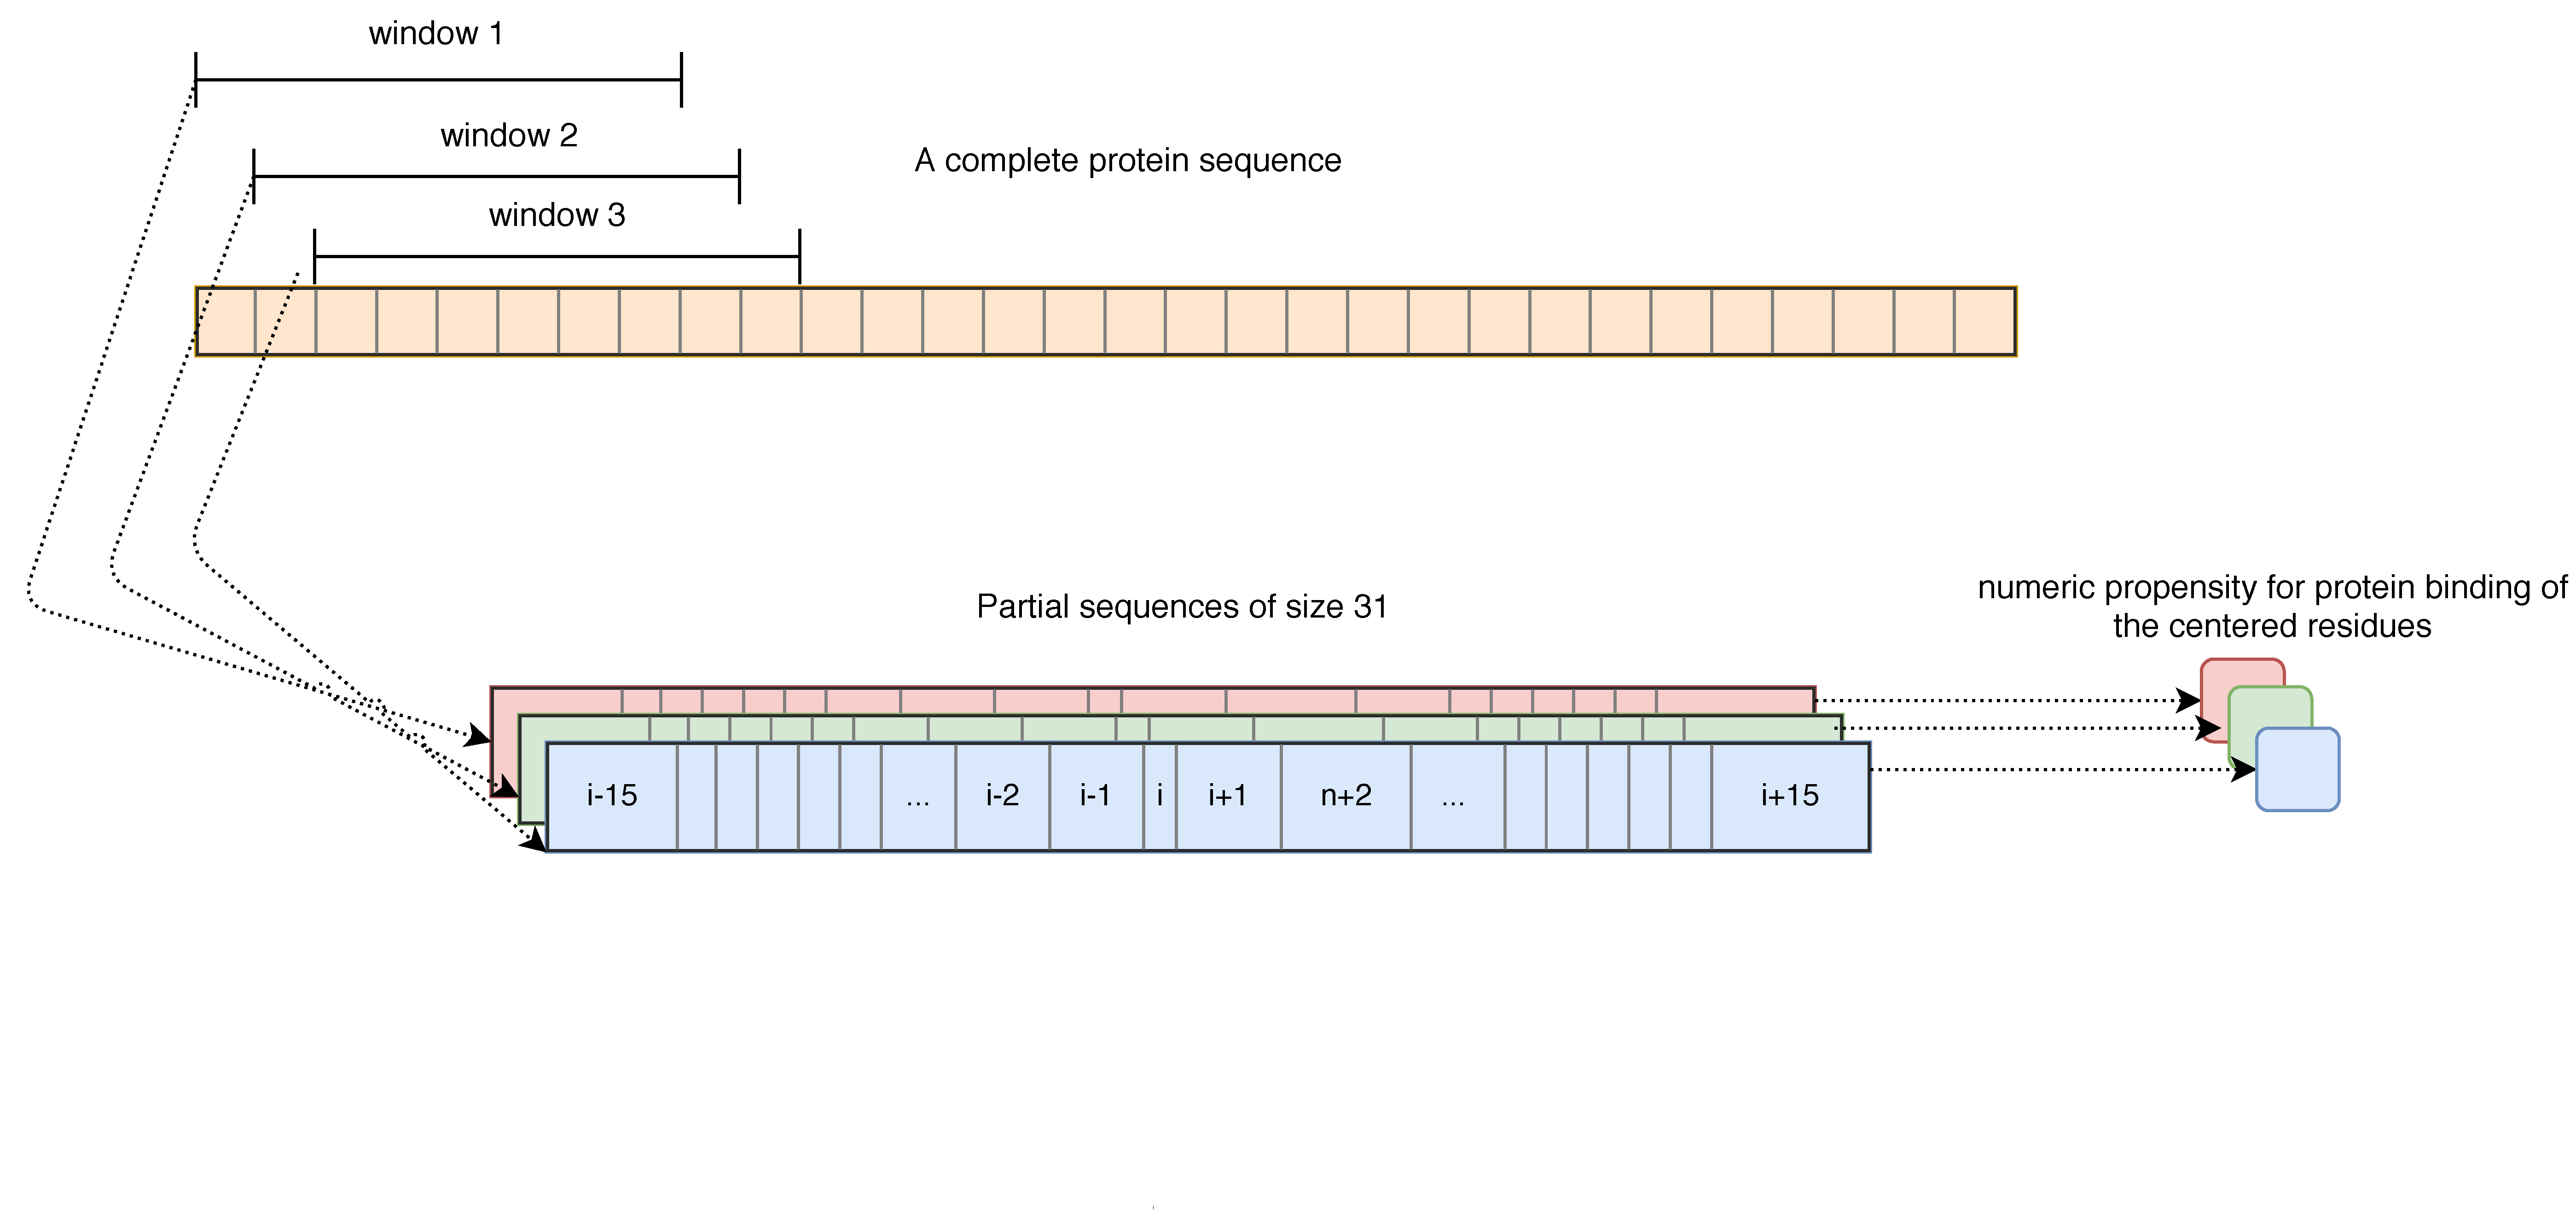
\includegraphics[width=\textwidth]{img/many_2_one.pdf}
  \caption{The many-to-one prediction. Sliding windows of size 31, stride 1 are put on top of an input protein sequence. Each time, a sub-sequence of length 31 is extracted. The model predicts the protein-binding propensity of the middle amino acid for each sub-sequence.
  \label{fig_many2one}}
\end{figure*}
\subsubsection{CNN component}
The CNN model one has a concise structure: one convolution layer, one maxpooling layer, one flatten layer, and two fully connected layers. For each input sub-sequence of size 31, a 2D feature profile of size 39 by 31 is constructed. The 2D vector is reshaped into 3D and then passed to a convolution 2D layer, followed by a maxpooling layer. The intuition of using the convolution and maxpooling layers is that a 2D protein profile vector can be considered as an image with one channel, and the CNN model captures the combination of several features in a partial image. The results are flattened and then fed into two fully connected layers with dropout for regularization. The last fully connected layer has one unit with activation function sigmoid, so that the output is a single value between 0 to 1. The higher the value, the more confident the CNN model claims that the residue is a PPI binding site.
\subsubsection{RNN component}
The RNN component has the following structure: one bidirectional GRU layer, one flatten layer, and two fully connected layers. Similar to the CNN component, a 2D feature profile of size 39 by 31 is built for each 31-mer. The feature profile is passed to a bidirectional gated recurrent units (GRU) layer with the intention to memories the dependency and relationship among the 31 residues. We set the GRU layer to return a whole sequence as opposed to return a single value. The results are flattened and fed into two fully connected layers with dropout. The output of the RNN network is also a single value between 0 to 1.
\subsubsection{Ensemble component}
The final model combines the core layers of the above mentioned CNN and RNN models and tries to further extract essential information of protein binding. The ensemble network takes a sequence of length 31 as its input. Similar to the CNN and RNN components, a 39 by 31 feature vector is constructed and passed to both a convolution layer and a bidirectional GRU layer. The output of the convolution layer is passed on to a maxpool layer and then flattened. The GRU output is also flattened. Then the outputs of the two flatten layers are concatenated and passed on to two fully connected layers with dropout. The last fully connected layer has one output unit with a sigmoid activation function, so the final output is a single value between 0 to 1, indicating the propensity of being binding sites. This is the final output of the entire model. 

Fine tuning is used in this ensemble model. The convolution layer in the CNN network and the bidirectional GRU layer in the RNN network are tuned separated using the same training/validation dataset. After achieving the best performance on the CNN and the RNN components, the weights of the convolution and the GRU layer are saved to files. In the ensemble model, the convolution and the GRU layer load the saved weights from the file and freeze the weights, so that during the process of training, the convolution and the GRU layer stay unchanged. Training and validation data are used again only to train the fully connected layers in the ensemble model. The code snippet on fine tuning is as follows.
\begin{lstlisting}[language=python,frame=single]
# initialize model checkpoint
mc = ModelCheckpoint("SavedModelAndWeights.h5",
monitor = 'val_loss', mode='min', save_best_only=True)
# save model and weights during training
model.fit([features, labels, callbacks=[mc]
# in the ensemble model, load weights for conlution and GRU
model.load_weights("SavedModelAndWeights", by_name=True)
\end{lstlisting}

\subsection{Parameter/Hyper-parameter Tuning}
Parameters and hyper-parameters are chosen based on the training dataset while applying early stopping \cite{prechelt1998early} on the validation set. As shown in Fig. \ref{fig_earlyStop}, early stopping halts the training process when a performance drop on the validation set is detected. This is to avoid overfitting the training dataset. The early stopping code snippet using Keras callbacks module is as follows.
\begin{figure}[!h]
\begin{center}
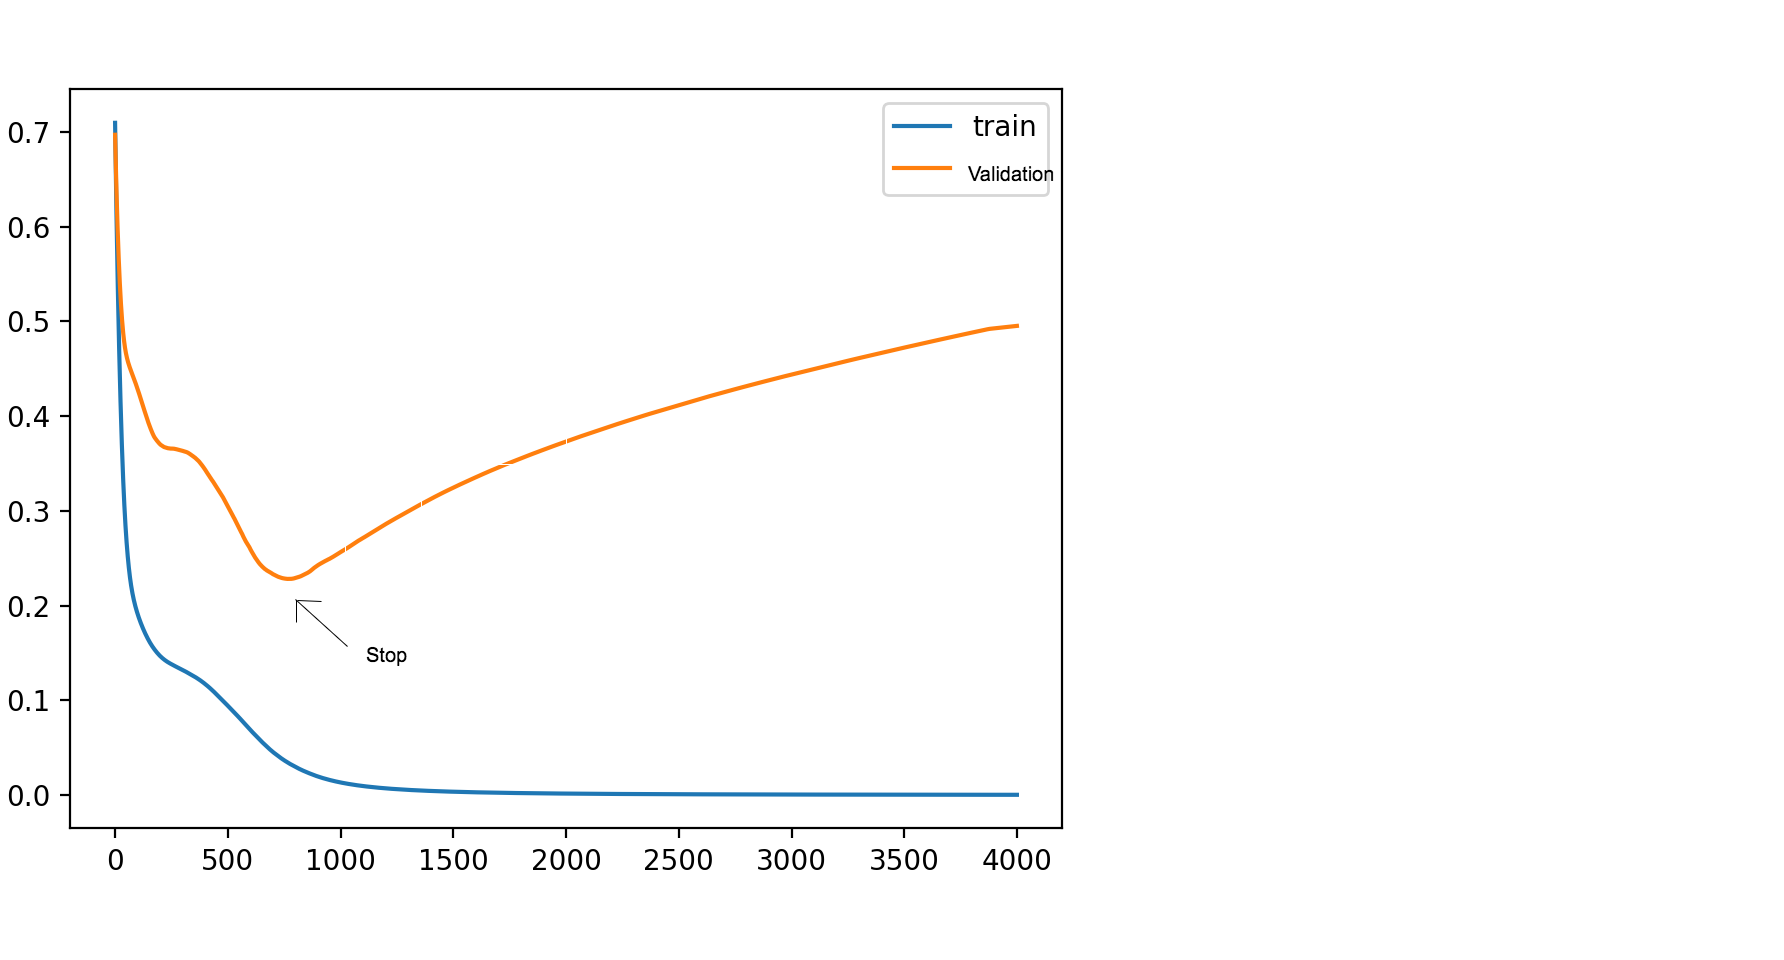
\includegraphics[width = 9cm]{img/early_stop.png}
\caption{Illustration of early stopping. The training process stops at the arrow point. The right side of the point is overfitting the training dataset. The left side of the point is underfitting. \label{fig_earlyStop}}
\end{center}
\end{figure}

\begin{lstlisting}[language=python,frame=single]
es = EarlyStopping(monitor='val_loss', mode='min', patience=4)
model.fit([features, labels, callbacks=[es]
\end{lstlisting}
We chose all parameters with the purpose to maximize area under the precision-recall curve (AUPRC) of the training data. All testing results are then carried using the already tuned model. All parameters and hyper-parameters used in this model are shown in Table \ref{tab_parameter}.

The DELPHI model takes 2.1 hours to train the CNN component, 0.5 hour to train the RNN component and 1.3 hours to train the ensemble model on our testing cluster.

% Table generated by Excel2LaTeX from sheet 'Sheet1'
\begin{table}[htbp]
  \centering
  \caption{Parameters used in DELPHI. Parameters are divided into four groups: CNN, RNN, ensemble model, and hyper-parameters.}
    \begin{tabular}{lr}
    Parameter & Value \\
    \midrule
    \midrule
    Epoch in CNN & 8 \\
    Kernel size in CNN & 5 \\
    Stride in CNN & 1 \\
    Padding in CNN & valid \\
    Number of filters in CNN & 64 \\
    Fully connected unit in CNN & 64, 1 \\
    \midrule
    Epoch in RNN & 9 \\
    GRU unit & 32 \\
    Fully connected unit in RNN & 64, 1 \\
    \midrule
    Epoch in ensemble & 5 \\
    Fully connected unit in ensemble & 96, 1 \\
    \midrule
    Batch size & 1024 \\
    Dropout rate & 0.3 \\
    Optimizer & Adam ($\beta_1=0.9, \beta_2=0.999$) \\
    Patience in early stop & 4 \\
    Loss function & binary cross entropy \\
    Learning rate & 0.002 \\
    \bottomrule
    \end{tabular}%
  \label{tab_parameter}%
\end{table}%
\subsection{Implementation}
Many open sourced programs in bioinformatics are not well written and maintained. It is frustrating for future researchers spending weeks even months just to compile and run a program. The engineering quality in academia is often compromised and forgiven. Indeed, research novelty is more important than good coding structure, git practise, and readability, but good engineering always plays a key role in successful projects. Projects like LLVM \cite{lattner2004llvm} and TensorFlow \cite{tensorflow2015-whitepaper} have thrived for years with huge open source communities not only because of the back scene innovational ideas, but also because of the excellent code base and infrastructure. We provide here some environment and implementation details hoping to help users to use DELPHI better, recreate results easier, and improve upon the current code base.

\subsubsection{Environment configuration}
System environment configuration is a step many researchers ignore or choose to do improperly. Each project has its unique compiler, package, and environmental variable settings. DevOp skills are not trivial for AI engineers without system configure experience. There are several solutions to ensure users running a program under the correct environment. Containers like docker is a complete industrial solution. Docker stores the entire operation system (OS) in an image, and the users can load the image such that the environment is identical. However, containers at the OS level is too heavy weighted. Lighter weighted solutions such as Python Virtual Environment, Anaconda are sufficient at package level, especially for python package management. According to GitHub statistics in 2019, about 50\% of the machine learning languages are written in Python.

DELPHI uses Python (3.5) Virtul Environment to manage all packages. Each virtual environment has its own packages and dependencies installed locally. Users can switch between any project environment without root permission nor modifying system directories. All packages needed by DELPHI is stored in Requirements.txt. The commands to creat the virtual environment for DELPHI are as follows.
\begin{lstlisting}[language=bash,frame=single]
# create a python3 environment
$ virtualenv -p [python3.5_path] [environment_name] 
# activate the newly created environment
$ source [environment_name]/bin/activate 
# install all packages neede by DELPHI
$ pip3 install -r Requirements.txt 
\end{lstlisting}

The DELPHI program is written in python, with Keras \cite{chollet2015keras} APIs and TensorFlow GPU back end. All features are computed from sequence only. We alleviate the burden of feature computation from users by providing all computation programs and a pipeline script. We ease the system configuration process by providing users a pip package list which enables one-command installation. 

\subsubsection{Class weights}
Classifying protein binding residue is an imbalanced problem. To cope with that, different class weights \cite{ting2002instance} are assigned to the positive and negative samples, so that the model pays more attention to the minority class, which is the binding sites.  The values are determined by the inverse of the class distribution in the training datasets. In our program, the weights are 0.55 and 4.97 for the non-binding and binding sites respectively. The code piece for implementing the class weights is as follows.
\begin{lstlisting}[language=python,frame=single,basicstyle=\small]
# compute the class weight in a balanced manner
cw = class_weight.compute_class_weight('balanced',
                np.unique(all_labels),all_labels)
# apply the class weights during training
model.fit(class_weight = cw, ...)
\end{lstlisting}

\subsubsection{Data shuffling}
During training, we shuffle the data before each epoch. Since the sliding window is used to extract each 31-mer, adjacent data entries are very similar; only the first and the last residue differ from the previous and the next data entry. Shuffling the whole training data diversifies the input in each batch. We experimentally trained the model with and without data shuffling, and shuffling the data rendered better predictions. This can be done by 
\begin{lstlisting}[language=python,frame=single]
  model.fit(shuffle=True, ...)
\end{lstlisting}

\section{Results}
We have comprehensively compared DELPHI with nine state-of-the-art machine learning based methods. The methods are selected using the following criteria. First, the program is a sequence-based method as sequence information is readily available for most proteins. Second, the program is available in the form of source code or web server. Lastly, the program takes in any input sequence in FASTA format and produces the results on an average-length protein within thirty minutes. Following these criteria, DLpred \cite{zhang2019sequence}, SCRIBER \cite{zhang2019scriber}, SSWRF \cite{wei2016protein}, SPRINT \cite{taherzadeh2016sequence}, CRF-PPI \cite{wei2015cascade}, LORIS \cite{dhole2014sequence}, SPRINGS \cite{singh2014springs}, PSIVER \cite{murakami2010applying}, and SPPIDER \cite{porollo2007prediction} are selected.

All competing methods are pre-trained using their own training and validation datasets. The most revent two programs, DLPred and SCRIBER, use 5719 and 843 training proteins respectively. The training dataset of DLPred is obtained from CullPDB datasets \cite{wang2003pisces} and further filtered by the authors. The SCRIBER training dataset is originally from the BioLip database. This dataset contains also protein binding information with DNA, RNA, and ligand, which is used by SCRIBER.

All tests have been performed on a Linux (Ubuntu 16.04) machine with 24 CPUs (Intel Xeon v4, 3.00GHz), 256GB memory, and a Nvidia Tesla K40c GPU.
\subsection{Datasets}
Five datasets are used in the comparative assessment. Four of them are publicly available dataset from previous studies: Dset\_186 \cite{murakami2010applying}, Dset\_72 \cite{hwang2008protein}, Dset\_164 \cite{dhole2014sequence}, and Dset\_448 \cite{zhang2019scriber}. The first three have been widely used and explored by previous studies while Dset\_448 is more recent. The raw data of Dset\_448 was from the BioLip database \cite{yang2012biolip} where binding sites are defined if the distance between an atom of a residues and an atom of a given protein partner <0.5 \AA{} plus the sum of the Van der Waals radii of the two atoms. The raw data was further processed by the authors of \cite{zhang2019scriber}, removing protein fragments, mapping BioLip sequences to UniProt sequences, clustering so that no similarities above 25\% is shared within the dataset. The number of sequences, binding, non-binding, and the ratio of binding residues are shown in Table \ref{tab_dataset}. The training dataset of DLPred has some overlaps with Dset\_448, therefore we removed 93 proteins in Dset\_448 that share more than 40\% similarities with DLPred training data and formed a reduced testing dataset of 355 proteins (Dset\_355).  According to the PSI-CD-HIT results, the training datasets of DLPred and SCRIBER still contain some proteins that share more than 25\% similarity to Dset\_186,  Dset\_72, and Dset\_164. However, we kept these testing datasets untouched because otherwise we would have to remove too many proteins from them. The training datasets of the competing programs can not be changed because the models are pre-trained. Note that all testing data share less than 25\% similarity to the training dataset of DELPHI. 

\begin{table*}[htbp]
    \centering
    \caption{The datasets used for training, validation, and testing. The first column gives the dataset names. The second column contains the number of proteins in each dataset. The third, fourth, and fifth columns represent the total number of residue, the number of binding, and the number of non-binding residues in each dataset. The last column represents the percentage of the binding residues out of total.}
    \begin{tabular}{p{12em}rrrrr}
    \toprule
    Dataset & Proteins & \multicolumn{3}{c}{Residues} & \multicolumn{1}{c}{\% binding} \\ \cline{3-5}
    & & total & binding & non-binding & \multicolumn{1}{c}{out of total}\\ \hline
    Dset\_448 & 448   & 116,500 & 15,810 & 100,690 & 13.57\% \\
    Dset\_355 & 355   & 95,940 & 11,467 & 84,473 & 11.95\% \\
    Dset\_186 & 186   & 36,219 & 5,517 & 30,702 & 15.23\% \\
    Dset\_72 & 72    & 18,140 & 1,923 & 16,217 & 10.60\% \\
    Dset\_164 & 164   & 33,681 & 6,096 & 27,585 & 18.10\% \\
    Training + validation & 9,982 & 4,254,198 & 427,687 & 3,826,511 & 10.05\% \\
    \hline
    \end{tabular}%
    \label{tab_dataset}%
\end{table*}%
\subsection{Evaluation Scheme}
Similar to previous studies, we use sensitivity, specificity, precision, accuracy, F1-measure, (F1), Matthews correlation coefficient (MCC), area under the receiver operating characteristic curve (AUROC), and area under the precision-recall (AUPRC) to measure the prediction performance. All programs output a prediction value for each amino acid, and thus the receiver operating characteristic (ROC) curve and the precision-recall (PR) curve can be drawn. AUROC and AUPRC are computed based on the curves using Scikit-learn~\cite{scikit-learn}. We focus more on AUROC and AUPR because they are threshold independent and convey an overall performance measurement of a program. The rest of the metrics are calculated using a binding threshold which is determined after obtaining the prediction scores from each program. Since each program's output is of different scale, for each program, we pick the threshold such that for a given testing dataset, the number of predicted scores above the threshold is equal to the real number of binding sites in the dataset. 

The formulas for calculating the metrics are as follows, where true positives ($TP$) and true negatives ($TN$) are the correctly predicted binding sites and non-binding sites, respectively, and false positives ($FP$) and false negative ($FN$) are incorrectly predicted binding sites and non-binding sites, respectively.
\begin{equation}
\textit{Sensitivity} = \frac{TP}{TP+FN}
\end{equation}

\begin{equation}
\textit{Specificity} = \frac{TN}{TN+FP}
\end{equation}

\begin{equation}
\textit{Precision} = \frac{TP}{TP + FP} 
\end{equation}

\begin{equation}
\textit{Accuracy}=\frac{TP+TN}{TP+FN+TN+FP}
\end{equation}

\begin{equation}
F1=2\times \frac{\textit{Sensitivity}\times \textit{Precision}}{\textit{Sensitivity}+\textit{Precision}}
\end{equation}

\begin{equation}
MCC\!=\!\frac{TP \times TN - FN \times FP}{\sqrt{(TP\!+\!FP)\!\times\! (TP\!+\!FN)\! \times \!(TN\!+\!FP)\!\times\!(TN\!+\!FN)}}
\end{equation}
\subsection{Comparative Analysis on Dset\_448}
We first compare the DELPHI model with eight programs on Dset\_448. This dataset is the most recently published and has the largest number of proteins, so we emphasize the importance of this dataset. As shown in Table~\ref{tab_comp_448}, DELPHI surpasses competitors in all metrics with an improvement of 3.08\% and 17.4\% on AUROC and AUPR respectively comparing to the second best program SCRIBER.

\begin{table*}[htbp]
  \centering
  \caption{Performance comparison of nine programs on Dset\_448. Programs are sorted in asending order by AUPRC. Darker colours represent better results. The evaluation of the programs marked with \** are carried by \cite{zhang2019scriber}.}
    % Table generated by Excel2LaTeX from sheet 'Sheet2'

    \begin{tabular}{lrrrrrrrr}
    \toprule
    \multicolumn{1}{|l}{Predictor} & \multicolumn{1}{c}{Sensitivity} & \multicolumn{1}{c}{Specificity} & \multicolumn{1}{c}{Precision} & \multicolumn{1}{c}{Accuracy} & \multicolumn{1}{c}{F1} & \multicolumn{1}{c}{MCC} & \multicolumn{1}{c}{AUROC} & \multicolumn{1}{c|}{AUPRC} \\
    \midrule
    \multicolumn{9}{|c|}{Dset\_448} \\
    \midrule
    SPPIDER* & \cellcolor[rgb]{ .933,  .953,  .922}0.202 & 0.870 & \cellcolor[rgb]{ .961,  .973,  .957}0.194 & 0.781 & \cellcolor[rgb]{ .949,  .965,  .937}0.198 & \cellcolor[rgb]{ .957,  .969,  .949}0.071 & 0.517 & 0.159 \\
    SPRINT* & 0.183 & \cellcolor[rgb]{ .937,  .953,  .925}0.873 & 0.183 & 0.781 & 0.183 & 0.057 & \cellcolor[rgb]{ .839,  .882,  .812}0.570 & \cellcolor[rgb]{ .973,  .98,  .965}0.167 \\
    PSIVER* & \cellcolor[rgb]{ .973,  .98,  .969}0.191 & \cellcolor[rgb]{ .918,  .937,  .902}0.874 & \cellcolor[rgb]{ .973,  .98,  .969}0.191 & \cellcolor[rgb]{ .973,  .98,  .969}0.783 & \cellcolor[rgb]{ .973,  .98,  .969}0.191 & \cellcolor[rgb]{ .973,  .98,  .969}0.066 & \cellcolor[rgb]{ .808,  .859,  .773}0.581 & \cellcolor[rgb]{ .961,  .973,  .953}0.170 \\
    SPRINGS* & \cellcolor[rgb]{ .839,  .882,  .808}0.229 & \cellcolor[rgb]{ .745,  .812,  .698}0.882 & \cellcolor[rgb]{ .843,  .886,  .812}0.228 & \cellcolor[rgb]{ .792,  .847,  .753}0.796 & \cellcolor[rgb]{ .839,  .882,  .808}0.229 & \cellcolor[rgb]{ .835,  .878,  .804}0.111 & \cellcolor[rgb]{ .675,  .761,  .612}0.625 & \cellcolor[rgb]{ .843,  .886,  .816}0.201 \\
    LORIS* & \cellcolor[rgb]{ .714,  .792,  .659}0.264 & \cellcolor[rgb]{ .635,  .733,  .569}0.887 & \cellcolor[rgb]{ .718,  .792,  .663}0.263 & \cellcolor[rgb]{ .667,  .757,  .604}0.805 & \cellcolor[rgb]{ .718,  .792,  .663}0.263 & \cellcolor[rgb]{ .71,  .788,  .655}0.151 & \cellcolor[rgb]{ .58,  .694,  .502}0.656 & \cellcolor[rgb]{ .741,  .812,  .694}0.228 \\
    CRFPPI* & \cellcolor[rgb]{ .698,  .78,  .643}0.268 & \cellcolor[rgb]{ .635,  .733,  .569}0.887 & \cellcolor[rgb]{ .714,  .792,  .659}0.264 & \cellcolor[rgb]{ .667,  .757,  .604}0.805 & \cellcolor[rgb]{ .706,  .784,  .651}0.266 & \cellcolor[rgb]{ .698,  .78,  .643}0.154 & \cellcolor[rgb]{ .502,  .635,  .412}0.681 & \cellcolor[rgb]{ .706,  .784,  .651}0.238 \\
    SSWRF* & \cellcolor[rgb]{ .627,  .729,  .561}0.288 & \cellcolor[rgb]{ .549,  .671,  .471}0.891 & \cellcolor[rgb]{ .635,  .733,  .569}0.286 & \cellcolor[rgb]{ .584,  .694,  .506}0.811 & \cellcolor[rgb]{ .631,  .729,  .565}0.287 & \cellcolor[rgb]{ .624,  .725,  .557}0.178 & \cellcolor[rgb]{ .482,  .624,  .388}0.687 & \cellcolor[rgb]{ .639,  .737,  .573}0.256 \\
    SCRIBER & \cellcolor[rgb]{ .463,  .608,  .365}0.334 & \cellcolor[rgb]{ .443,  .592,  .341}0.896 & \cellcolor[rgb]{ .471,  .612,  .373}0.332 & \cellcolor[rgb]{ .443,  .592,  .341}0.821 & \cellcolor[rgb]{ .467,  .612,  .369}0.333 & \cellcolor[rgb]{ .463,  .608,  .365}0.230 & \cellcolor[rgb]{ .4,  .561,  .29}0.715 & \cellcolor[rgb]{ .522,  .651,  .435}0.287 \\
    DELPHI & \cellcolor[rgb]{ .329,  .51,  .208}0.371 & \cellcolor[rgb]{ .329,  .51,  .208}0.901 & \cellcolor[rgb]{ .329,  .51,  .208}0.371 & \cellcolor[rgb]{ .329,  .51,  .208}0.829 & \cellcolor[rgb]{ .329,  .51,  .208}0.371 & \cellcolor[rgb]{ .329,  .51,  .208}0.272 & \cellcolor[rgb]{ .329,  .51,  .208}0.737 & \cellcolor[rgb]{ .329,  .51,  .208}0.337 \\
    \end{tabular}%
  \label{tab_comp_448}%
\end{table*}%

In order to have a more comprehensive comparison, we compare DELPHI with another recent sequence-based program, DLPred. However, the training data in DLPred has a big overlap with Dset\_448, so we removed the highly similar sequence in Dset\_448 using the protocol described in section \ref{testing_data} and produced a reduced dataset Dset\_355 which is tested in Section \ref{section_four_tests}. 

\subsection{Comparative Analysis on Dset\_355, Dset\_186, Dset\_164, and Dset\_72}
To further compare DELPHI with other programs, we used Dset\_355 along with another three previously published datasets: Dset\_186, Dset\_164, and Dset\_72. Since DLPred and SCRIBER are the most recent programs and have been shown to outperform older programs, we compare DELPHI only with SCRIBER and DLPred on the remaining datasets. As shown in Table \ref{tab_ds355_ds186_164_72}, DELPHI clearly outperforms the competitors in all metrics on all datasets it shares the least similarities to the testing datasets. As binding site prediction is a highly imbalanced task, the area under the PR curve is a better indication of the performance as it emphasises more on the minority class and ROC curve pays attention to both minority and the majority class \cite{andluis2016survey}. The AUPR is improved by 18.5\%, 10.0\%, 0.6\%, 10.2\% comparing to the second best program on each dataset. We present also the average values over Dset\_355, Dset\_186, Dset\_164, and Dset\_72 in Table \ref{tab_ds355_ds186_164_72} for each specificity value. The performance of DELPHI again surpasses all competing programs. The average AUPR improvement is 9.7\%.  
\begin{table*}
  \centering
  \caption{Performance comparison of SCRIBER, DLPred, and DELPHI on Dset\_355, Dset\_186, Dset\_164, and Dset\_72. Darker colours represent better results. Each dataset is tested separately using the same metrics. The average metrics of the three datasets is also shown.}
    \begin{tabular}{|lrrrrrrrr|}
    \toprule
    Predictor & \multicolumn{1}{c}{Sensitivity} & \multicolumn{1}{c}{Specificity} & \multicolumn{1}{c}{Precision} & \multicolumn{1}{c}{Accuracy} & \multicolumn{1}{c}{F1} & \multicolumn{1}{c}{MCC} & \multicolumn{1}{c}{AUROC} & \multicolumn{1}{c|}{AUPRC} \\
    \midrule
    \multicolumn{9}{|c|}{Dset\_355} \\
    \midrule
    SCRIBER & \cellcolor[rgb]{ .835,  .882,  .808}0.322 & \cellcolor[rgb]{ .847,  .886,  .816}0.908 & \cellcolor[rgb]{ .839,  .882,  .808}0.322 & \cellcolor[rgb]{ .847,  .89,  .82}0.838 & \cellcolor[rgb]{ .839,  .882,  .808}0.322 & \cellcolor[rgb]{ .839,  .882,  .808}0.230 & 0.719 & \cellcolor[rgb]{ .961,  .973,  .953}0.275 \\
    DLPred & 0.308 & 0.906 & 0.308 & 0.835 & 0.308 & 0.214 & \cellcolor[rgb]{ .89,  .922,  .871}0.724 & 0.272 \\
    DELPHI & \cellcolor[rgb]{ .329,  .51,  .208}0.364 & \cellcolor[rgb]{ .329,  .51,  .208}0.914 & \cellcolor[rgb]{ .329,  .51,  .208}0.364 & \cellcolor[rgb]{ .329,  .51,  .208}0.848 & \cellcolor[rgb]{ .329,  .51,  .208}0.364 & \cellcolor[rgb]{ .329,  .51,  .208}0.278 & \cellcolor[rgb]{ .329,  .51,  .208}0.746 & \cellcolor[rgb]{ .329,  .51,  .208}0.326 \\
    \midrule
    \multicolumn{9}{|c|}{Dset\_186} \\
    \midrule
    SCRIBER & 0.279 & 0.870 & 0.279 & 0.780 & 0.279 & 0.150 & 0.647 & 0.246 \\
    DLPred & \cellcolor[rgb]{ .62,  .722,  .549}0.320 & \cellcolor[rgb]{ .631,  .729,  .565}0.878 & \cellcolor[rgb]{ .62,  .722,  .549}0.320 & \cellcolor[rgb]{ .631,  .729,  .561}0.793 & \cellcolor[rgb]{ .62,  .722,  .549}0.320 & \cellcolor[rgb]{ .62,  .722,  .553}0.198 & \cellcolor[rgb]{ .498,  .631,  .404}0.694 & \cellcolor[rgb]{ .6,  .71,  .529}0.290 \\
    DELPHI & \cellcolor[rgb]{ .329,  .51,  .208}0.351 & \cellcolor[rgb]{ .329,  .51,  .208}0.884 & \cellcolor[rgb]{ .329,  .51,  .208}0.351 & \cellcolor[rgb]{ .329,  .51,  .208}0.803 & \cellcolor[rgb]{ .329,  .51,  .208}0.351 & \cellcolor[rgb]{ .329,  .51,  .208}0.235 & \cellcolor[rgb]{ .329,  .51,  .208}0.710 & \cellcolor[rgb]{ .329,  .51,  .208}0.319 \\
    \midrule
    \multicolumn{9}{|c|}{Dset\_164} \\
    \midrule
    SCRIBER & 0.327 & 0.851 & 0.327 & 0.756 & 0.327 & 0.179 & 0.657 & 0.301 \\
    DLPred & \cellcolor[rgb]{ .714,  .792,  .663}0.338 & \cellcolor[rgb]{ .71,  .788,  .659}0.854 & \cellcolor[rgb]{ .714,  .792,  .663}0.338 & \cellcolor[rgb]{ .714,  .788,  .659}0.760 & \cellcolor[rgb]{ .714,  .792,  .663}0.338 & \cellcolor[rgb]{ .714,  .792,  .663}0.192 & \cellcolor[rgb]{ .635,  .733,  .569}0.672 & \cellcolor[rgb]{ .365,  .537,  .251}0.330 \\
    DELPHI & \cellcolor[rgb]{ .329,  .51,  .208}0.352 & \cellcolor[rgb]{ .329,  .51,  .208}0.857 & \cellcolor[rgb]{ .329,  .51,  .208}0.352 & \cellcolor[rgb]{ .329,  .51,  .208}0.765 & \cellcolor[rgb]{ .329,  .51,  .208}0.352 & \cellcolor[rgb]{ .329,  .51,  .208}0.209 & \cellcolor[rgb]{ .329,  .51,  .208}0.685 & \cellcolor[rgb]{ .329,  .51,  .208}0.332 \\
    \midrule
    \multicolumn{9}{|c|}{Dset\_72} \\
    \midrule
    SCRIBER & 0.232 & \cellcolor[rgb]{ .612,  .718,  .541}0.909 & 0.232 & \cellcolor[rgb]{ .635,  .733,  .569}0.837 & 0.232 & 0.141 & 0.680 & 0.198 \\
    DLPred & \cellcolor[rgb]{ .776,  .839,  .737}0.246 & 0.901 & \cellcolor[rgb]{ .776,  .839,  .737}0.246 & 0.826 & \cellcolor[rgb]{ .776,  .839,  .737}0.246 & \cellcolor[rgb]{ .91,  .937,  .894}0.148 & \cellcolor[rgb]{ .82,  .867,  .784}0.688 & \cellcolor[rgb]{ .706,  .784,  .651}0.215 \\
    DELPHI & \cellcolor[rgb]{ .329,  .51,  .208}0.274 & \cellcolor[rgb]{ .329,  .51,  .208}0.914 & \cellcolor[rgb]{ .329,  .51,  .208}0.274 & \cellcolor[rgb]{ .329,  .51,  .208}0.847 & \cellcolor[rgb]{ .329,  .51,  .208}0.274 & \cellcolor[rgb]{ .329,  .51,  .208}0.189 & \cellcolor[rgb]{ .329,  .51,  .208}0.711 & \cellcolor[rgb]{ .329,  .51,  .208}0.237 \\
    \midrule
    \multicolumn{9}{|c|}{Average} \\
    \midrule
    SCRIBER & 0.290 & 0.885 & 0.290 & 0.803 & 0.290 & 0.175 & 0.676 & 0.255 \\
    DLPred & \cellcolor[rgb]{ .812,  .863,  .776}0.303 & \cellcolor[rgb]{ .992,  .992,  .988}0.885 & \cellcolor[rgb]{ .808,  .859,  .773}0.303 & \cellcolor[rgb]{ .976,  .984,  .973}0.803 & \cellcolor[rgb]{ .808,  .863,  .773}0.303 & \cellcolor[rgb]{ .835,  .882,  .804}0.188 & \cellcolor[rgb]{ .659,  .753,  .6}0.695 & \cellcolor[rgb]{ .702,  .784,  .647}0.277 \\
    DELPHI & \cellcolor[rgb]{ .329,  .51,  .208}0.335 & \cellcolor[rgb]{ .329,  .51,  .208}0.892 & \cellcolor[rgb]{ .329,  .51,  .208}0.335 & \cellcolor[rgb]{ .329,  .51,  .208}0.816 & \cellcolor[rgb]{ .329,  .51,  .208}0.335 & \cellcolor[rgb]{ .329,  .51,  .208}0.227 & \cellcolor[rgb]{ .329,  .51,  .208}0.713 & \cellcolor[rgb]{ .329,  .51,  .208}0.304 \\
    \bottomrule\label{tab_ds355_ds186_164_72}
    \end{tabular}%
\end{table*}%

\subsection{Feature Evaluation}
We conducted an another experiment to show that all twelve feature are necessary for DELPHI. We pruned one feature each time, and the remaining eleven features are used to train and then evaluate the DELPHI model. As shown in Fig. \ref{fig_remove_each_feature}, the performance decreases with the removal of any feature, showing that there are no redundant features. It is perhaps expected that  removing PSSM creates the biggest performance drop, but our newly introduced features, HSP, ProtVec1D, and Position are shown to be  very useful as well. 
\begin{figure}[!h]
\begin{center}
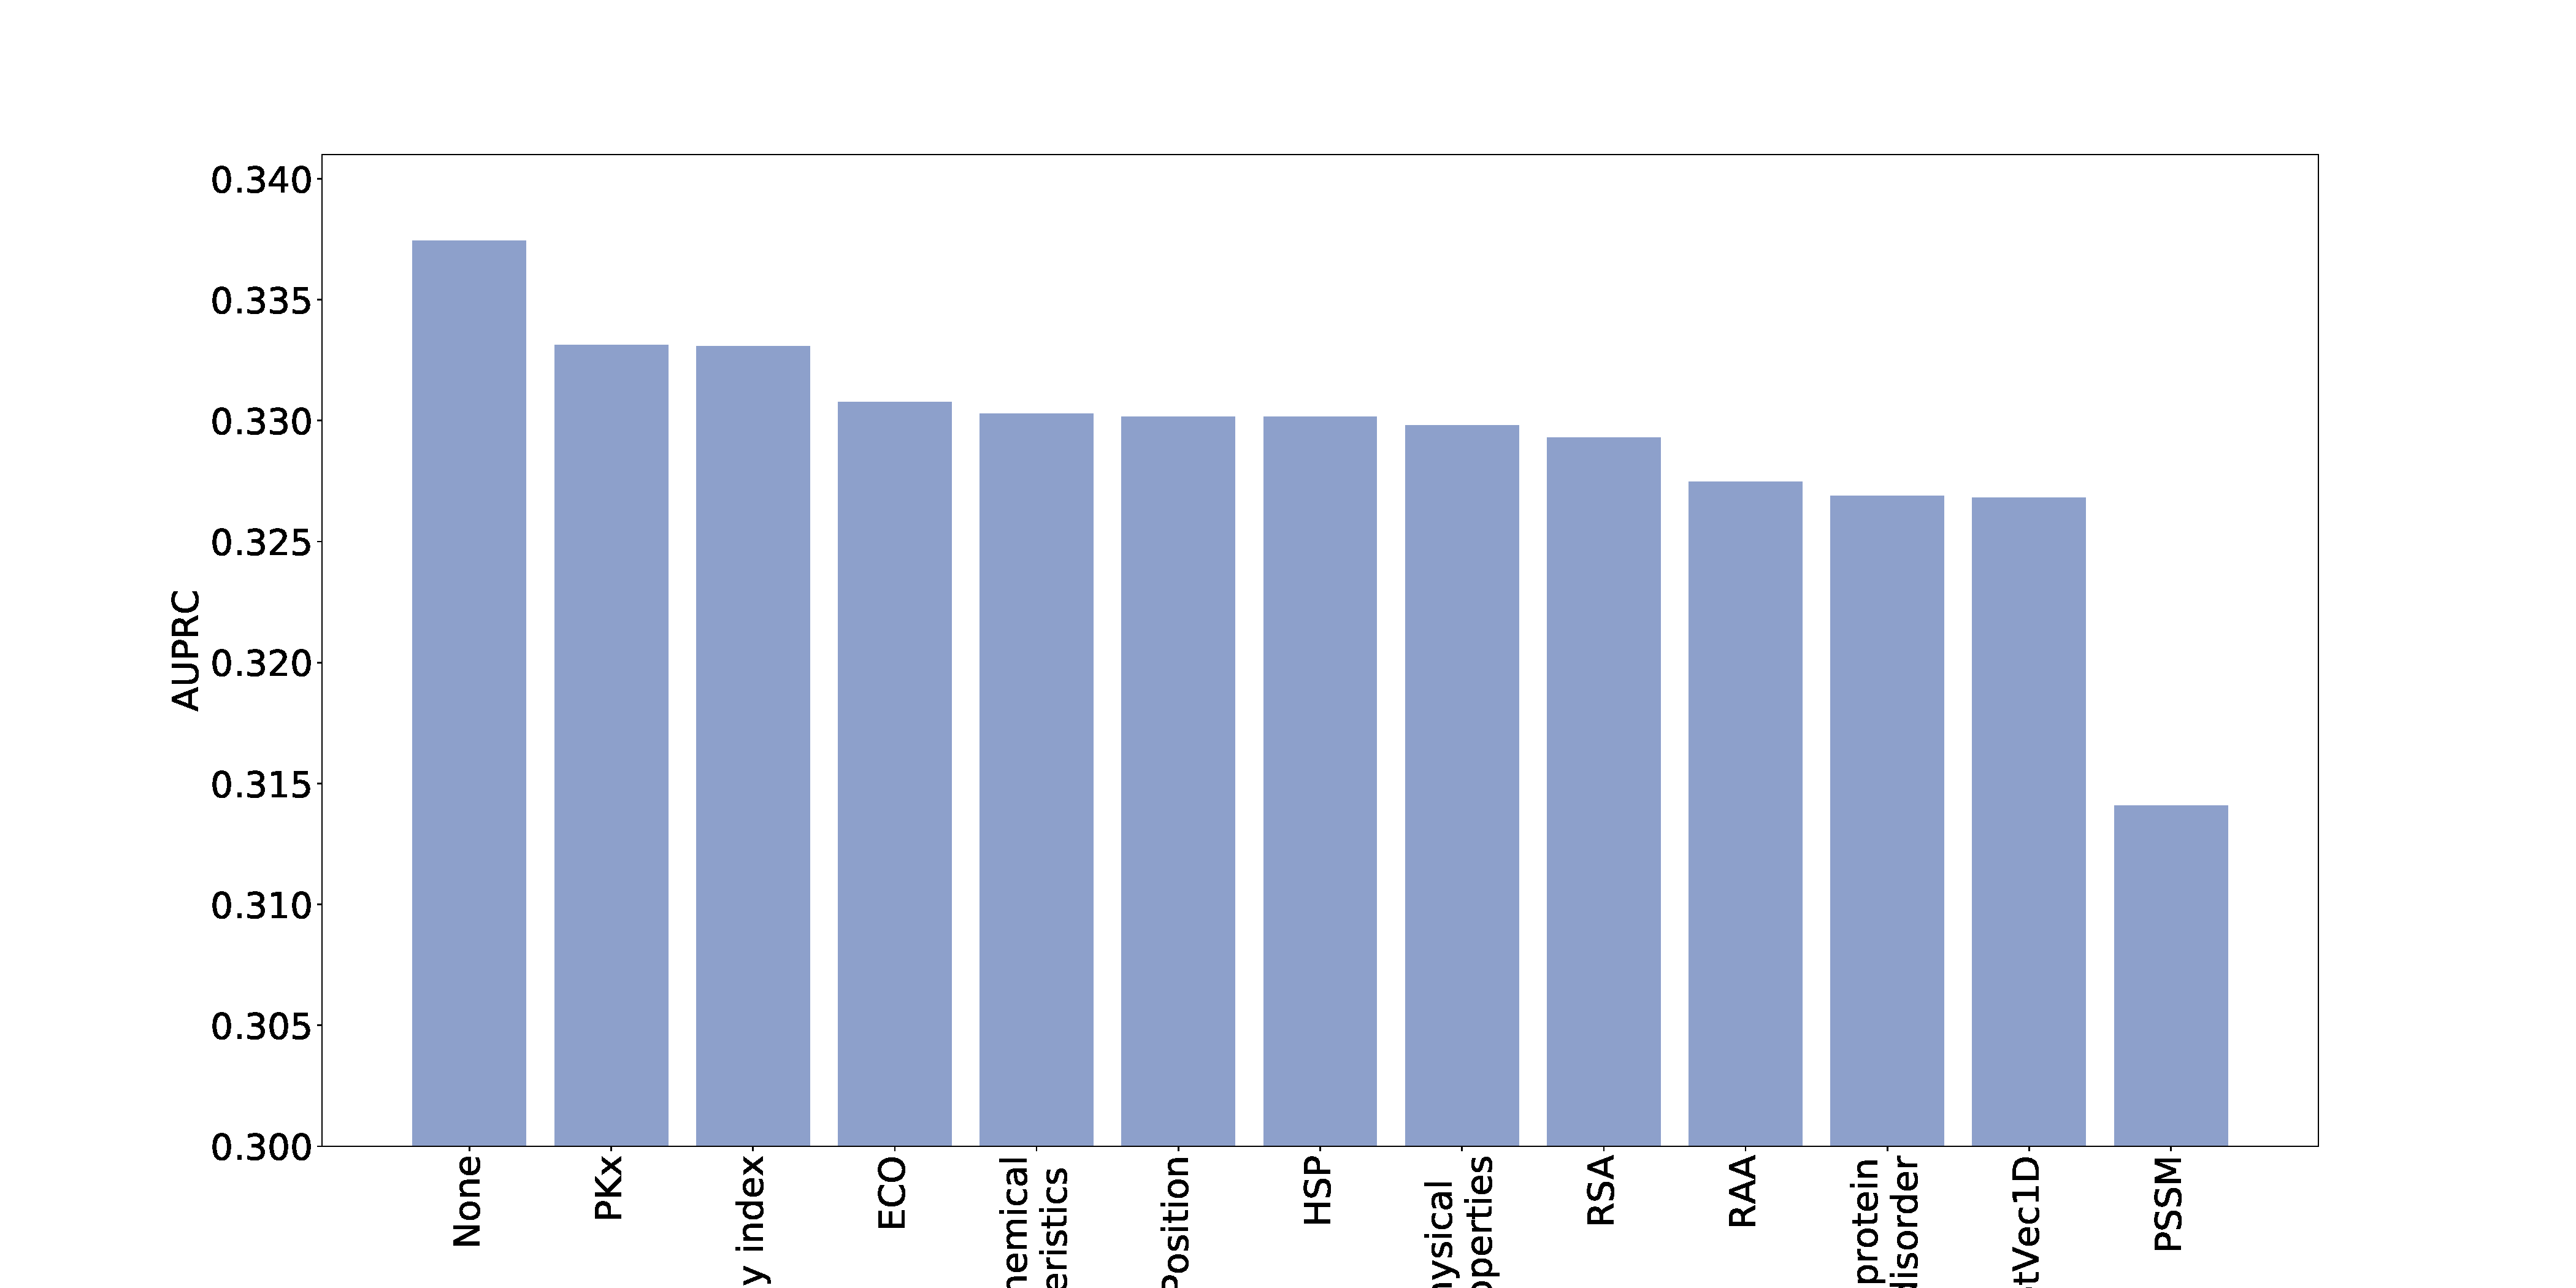
\includegraphics[height = 7cm, width = 9cm]{img/remove_features_individually_Testing.pdf}
\caption{The areas under PR curves with the removal of one out of the twelve features on Dset\_448. One feature is removed each time, and the DELPHI model is trained, validated, and tested using the remaining eleven features. The x-axis shows the removed features where 'None' indicates using all twelve features, and the y-axis is the AUPR achieved. The features are sorted by the AUPR values. } \label{fig_remove_each_feature}
\end{center}
\end{figure}

\subsection{Availability}
DELPHI is an open source program under the GPLv3 License. The trained model, source code of training, predicting, and data processing is freely available at\\ \texttt{https://github.comlucian-ilie/DELPHI}. 
All datasets used in this study can be downloaded at \texttt{http://www.csd.uwo.ca/\~{}ilie/DELPHI/}.\\
\section{Conclusion}
We introduced our program DELPHI and comprehensively compared it with nine state-of-the-art programs on five datasets. DELPHI provides the best predictions in all metrics. The contributions of the DELPHI study are as follows.
First, a novel fine tuned ensemble model combing CNN and RNN is constructed in which three features are used the first time in this problem. Second, a many-to-one structure, that not only serves as a data augmentation technique but also improves the prediction performance, is applied. Third, a data processing and feature construction suite, including new features, is provided, aiming to alleviating the difficulty of tedious feature computation by the users.